\documentclass[12pt]{article}

\usepackage[portuguese]{babel}
\usepackage[utf8]{inputenc}
\usepackage{amsmath}
\usepackage{commath}
\usepackage[alf]{abntex2cite}
\usepackage{indentfirst}
\usepackage{graphicx}
\usepackage{multicol,lipsum}
\usepackage{subfig}
\usepackage{geometry}
\usepackage[alf]{abntex2cite}
\usepackage{subfig}

\geometry{
	paper = a4paper,
    inner = 3cm,
    outer = 3cm,
    top = 2cm,
    bottom = 2cm
}

\begin{document}
%\maketitle

\onehalfspacing

\begin{titlepage}
	\begin{center}

		\Huge{Universidade Federal de Alagoas}\\
		\large{Instituto de Computação}\\ 
		\large{Laboratório de Computação Científica e Análise Numérica}\\ 
        \vspace{220pt}
        \textbf{\LARGE{Relatório de acompanhamento de pesquisa}}\\
		%\title{{\large{Título}}}
		\vspace{3,5cm}
	\end{center}
	
	\begin{flushleft}
		\begin{tabbing}
			Aluno: Danilo Fernandes Costa\\
			Professor orientador: Alejandro Frery\\
	\end{tabbing}
 \end{flushleft}
	\vspace{1cm}
	
	\begin{center}
		\vspace{\fill}
			 Fevereiro\\
		 2019
			\end{center}
\end{titlepage}

\section{Introdução}

No presente relatório são apresentados alguns resultados obtidos da análise de regiões de solo com pouca ou nenhuma vegetação. Os dados PolSAR das regiões analisadas foram extraídas de uma imagem da Sierra del Lacandon National Park, Guatemala a qual foi adquirida em 10 de abril de 2015. Segue as imagens das regiões analisidas:

\begin{figure}[hbt]
    \centering
    \subfloat[Região 1]{{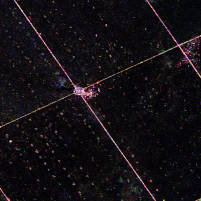
\includegraphics[width=0.4\linewidth]{../../Images/Report_19_02_27/ground_region1.png} }}%
    \qquad
    \subfloat[Região 2]{{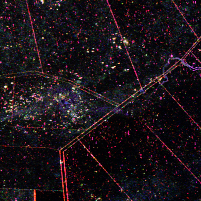
\includegraphics[width=0.4\linewidth]{../../Images/Report_19_02_27/ground_region2.png} }}%
    \vspace{0.05\linewidth}
    \subfloat[Região 3]{{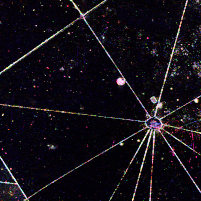
\includegraphics[width=0.4\linewidth]{../../Images/Report_19_02_27/ground_region3.png} }}%
    \qquad
    \subfloat[Região 4]{{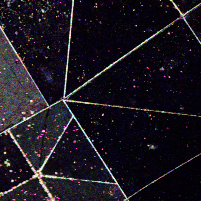
\includegraphics[width=0.4\linewidth]{../../Images/Report_19_02_27/ground_region4.png} }}%
    \caption{Regiões analisadas}
    \label{fig:regions}
\end{figure}
\newpage

Considerando a relação existente entre a decomposição de Pauli e regiões de vegetação em imagens PolSAR, obteve-se as imagens dessas regiões por meio dessa decomposição. Seguem as mesmas:

\begin{figure}[hbt]
    \centering
    \subfloat[Região 1]{{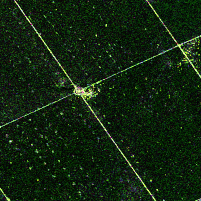
\includegraphics[width=0.4\linewidth]{../../Images/Report_19_02_27/guatemala_region1.png} }}%
    \qquad
    \subfloat[Região 2]{{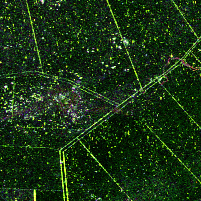
\includegraphics[width=0.4\linewidth]{../../Images/Report_19_02_27/guatemala_region2.png} }}%
    \vspace{0.05\linewidth}
    \subfloat[Região 3]{{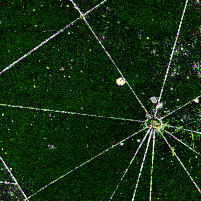
\includegraphics[width=0.4\linewidth]{../../Images/Report_19_02_27/guatemala_region3.png} }}%
    \qquad
    \subfloat[Região 4]{{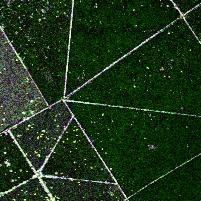
\includegraphics[width=0.4\linewidth]{../../Images/Report_19_02_27/guatemala_region4.png} }}%
    \caption{Regiões analisadas por meio da decomposição de Pauli}
    \label{fig:regions_pauli}
\end{figure}

Para fins de validação dos resultados obtidos, também obteve-se imagens de satélite ótico das regiões 1 e 2 e imagens de regiões vizinhas às regiões 3 e 4 no Google Earth as quais foram obtidas por esse em 27 de abril de 2015 -- 17 dias após a obtenção da imagem PolSAR analisada. Considerou-se regiões vizinhas às regiões 3 e 4 devido à indisponibilidade dessas na referida data (as mais próximas temporalmente datavam de 13 de fevereiro de 2013) e por apresentarem visualmente na imagem PolSAR gerada a mesma textura. Essas imagens estão a seguir e nestas é observável que as duas primeiras apresentam alguma vegetação, enquanto as duas últimas consistem em solo exposto.

\newpage
\begin{figure}[hbt]
    \centering
    \subfloat[Região 1]{{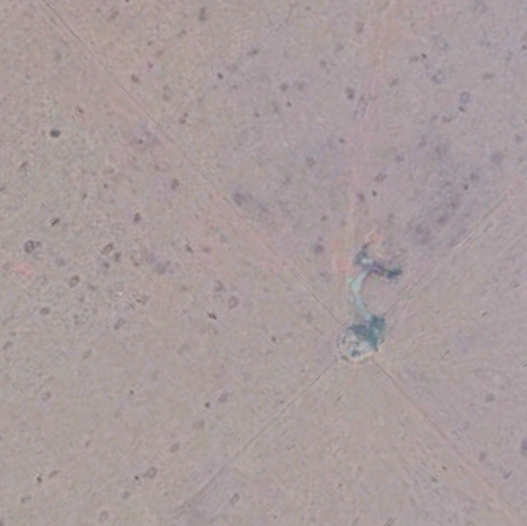
\includegraphics[width=0.4\linewidth]{../../Images/Report_19_02_27/optical_region1.png} }}%
    \qquad
    \subfloat[Região 2]{{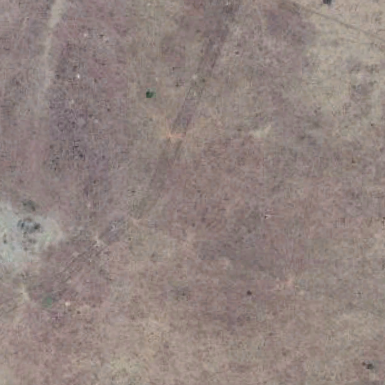
\includegraphics[width=0.4\linewidth]{../../Images/Report_19_02_27/optical_region2.png} }}%
    \vspace{0.05\linewidth}
    \subfloat[Região viznha à região 3]{{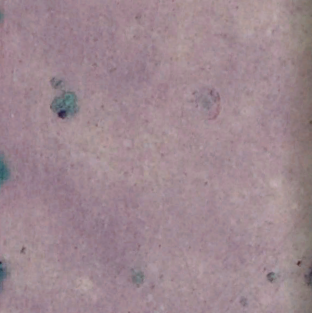
\includegraphics[width=0.4\linewidth]{../../Images/Report_19_02_27/optical_region3.png} }}%
    \qquad
    \subfloat[Região viznha à região 4]{{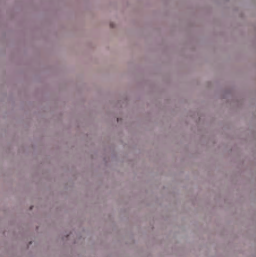
\includegraphics[width=0.4\linewidth]{../../Images/Report_19_02_27/optical_region4.png} }}%
    \caption{Regiões analisadas ou vizinhas obtidas por meio do Google Earth}
    \label{fig:regions_google_earth}
\end{figure}


%%% ACF Acrescentar a imagem correspondente do Google Earth
%%% ACF Visualizar em Pauli

\section{Análise das regiões}

Inicialmente analisou-se nas regiões quais retroespalhadores apresentavam maior similaridade a seus dados. Para tal analisou-se o mapa de retroespalhadores elementares, o qual atribui a cada \textit{pixel} o retroespalhador elementar mais próximo em relação à distância geodésica, para cada uma das regiões -- os quais são apresentados na figuras \ref{fig:scatterer_map1} à \ref{fig:scatterer_map4} -- e constatou-se que \textit{random volume} é predominante.

\begin{figure}[!h]

  \centering
  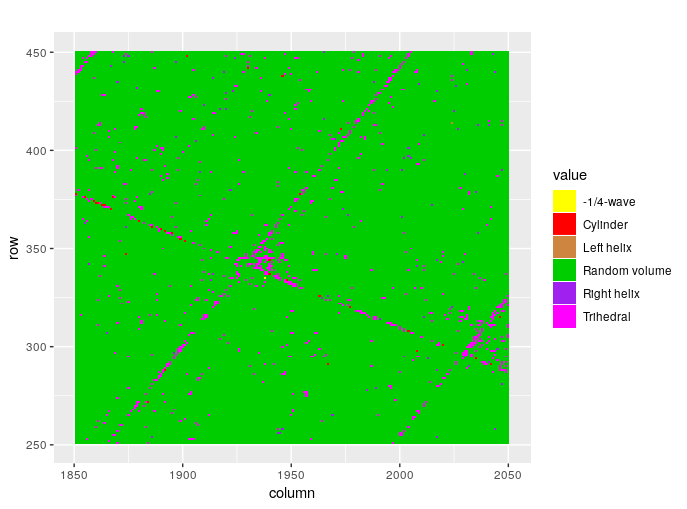
\includegraphics[width=\linewidth]{../../Images/Report_19_02_27/scatterer_map_region1.png}
  \caption{Mapa de retroespalhadores elementares da região 1}
  \label{fig:scatterer_map1}

\end{figure}

\begin{figure}[!h]

  \centering
  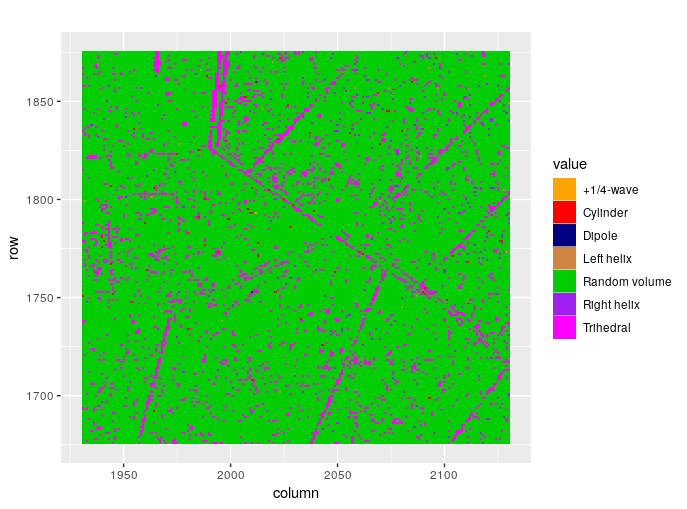
\includegraphics[width=\linewidth]{../../Images/Report_19_02_27/scatterer_map_region2.png}
  \caption{Mapa de retroespalhadores elementares da região 2}
  \label{fig:scatterer_map2}

\end{figure}

\newpage

\begin{figure}[!h]

  \centering
  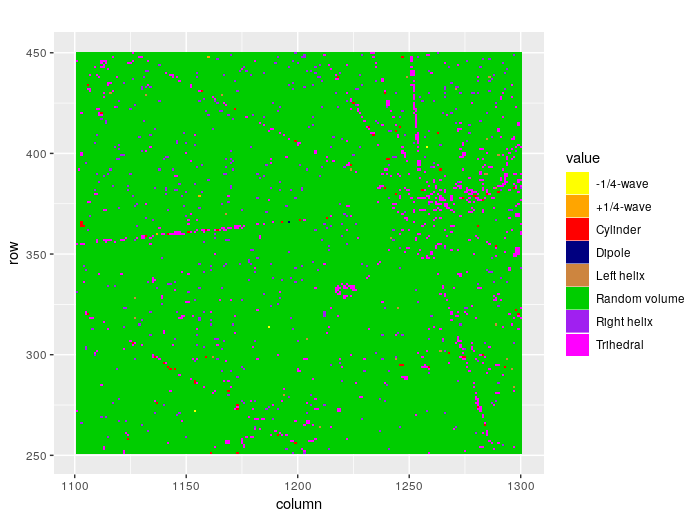
\includegraphics[width=\linewidth]{../../Images/Report_19_02_27/scatterer_map_region3.png}
  \caption{Mapa de retroespalhadores elementares da região 3}
  \label{fig:scatterer_map3}

\end{figure}

\begin{figure}[!h]

  \centering
  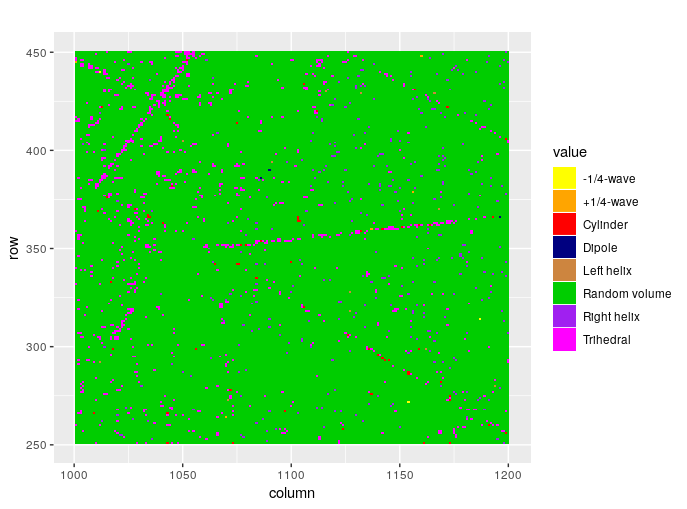
\includegraphics[width=\linewidth]{../../Images/Report_19_02_27/scatterer_map_region4.png}
  \caption{Mapa de retroespalhadores elementares da região 4}
  \label{fig:scatterer_map4}

\end{figure}

\newpage

Ao analisar-se os histogramas das similaridades dos dados mais próximos a \textit{random volume} em relação a este das regiões 1 e 2, os quais apresentam-se nas figuras \ref{fig:hist_beta_rv1} e \ref{fig:hist_beta_rv2}, observou-se a semelhança entre os histogramas e o ajuste a distribuição Beta. Para obter maior confiabilidade nesta observação, obteve-se os seus respectivos \textit{qqplots}, apresentados nas figuras \ref{fig:qqplot_beta_rv1} e \ref{fig:qqplot_beta_rv2}, os quais reinteram o afirmado.

%%% ACF Acrescentar tabela com # amostras, aplicar teste de aderência (Kolmogorov-Smirnov e chi-quadrado, informando o p-valor), ajustar dados por classe, informar parâmetros ajustados (nas duas parametrizações)

\begin{figure}[!h]

  \centering
  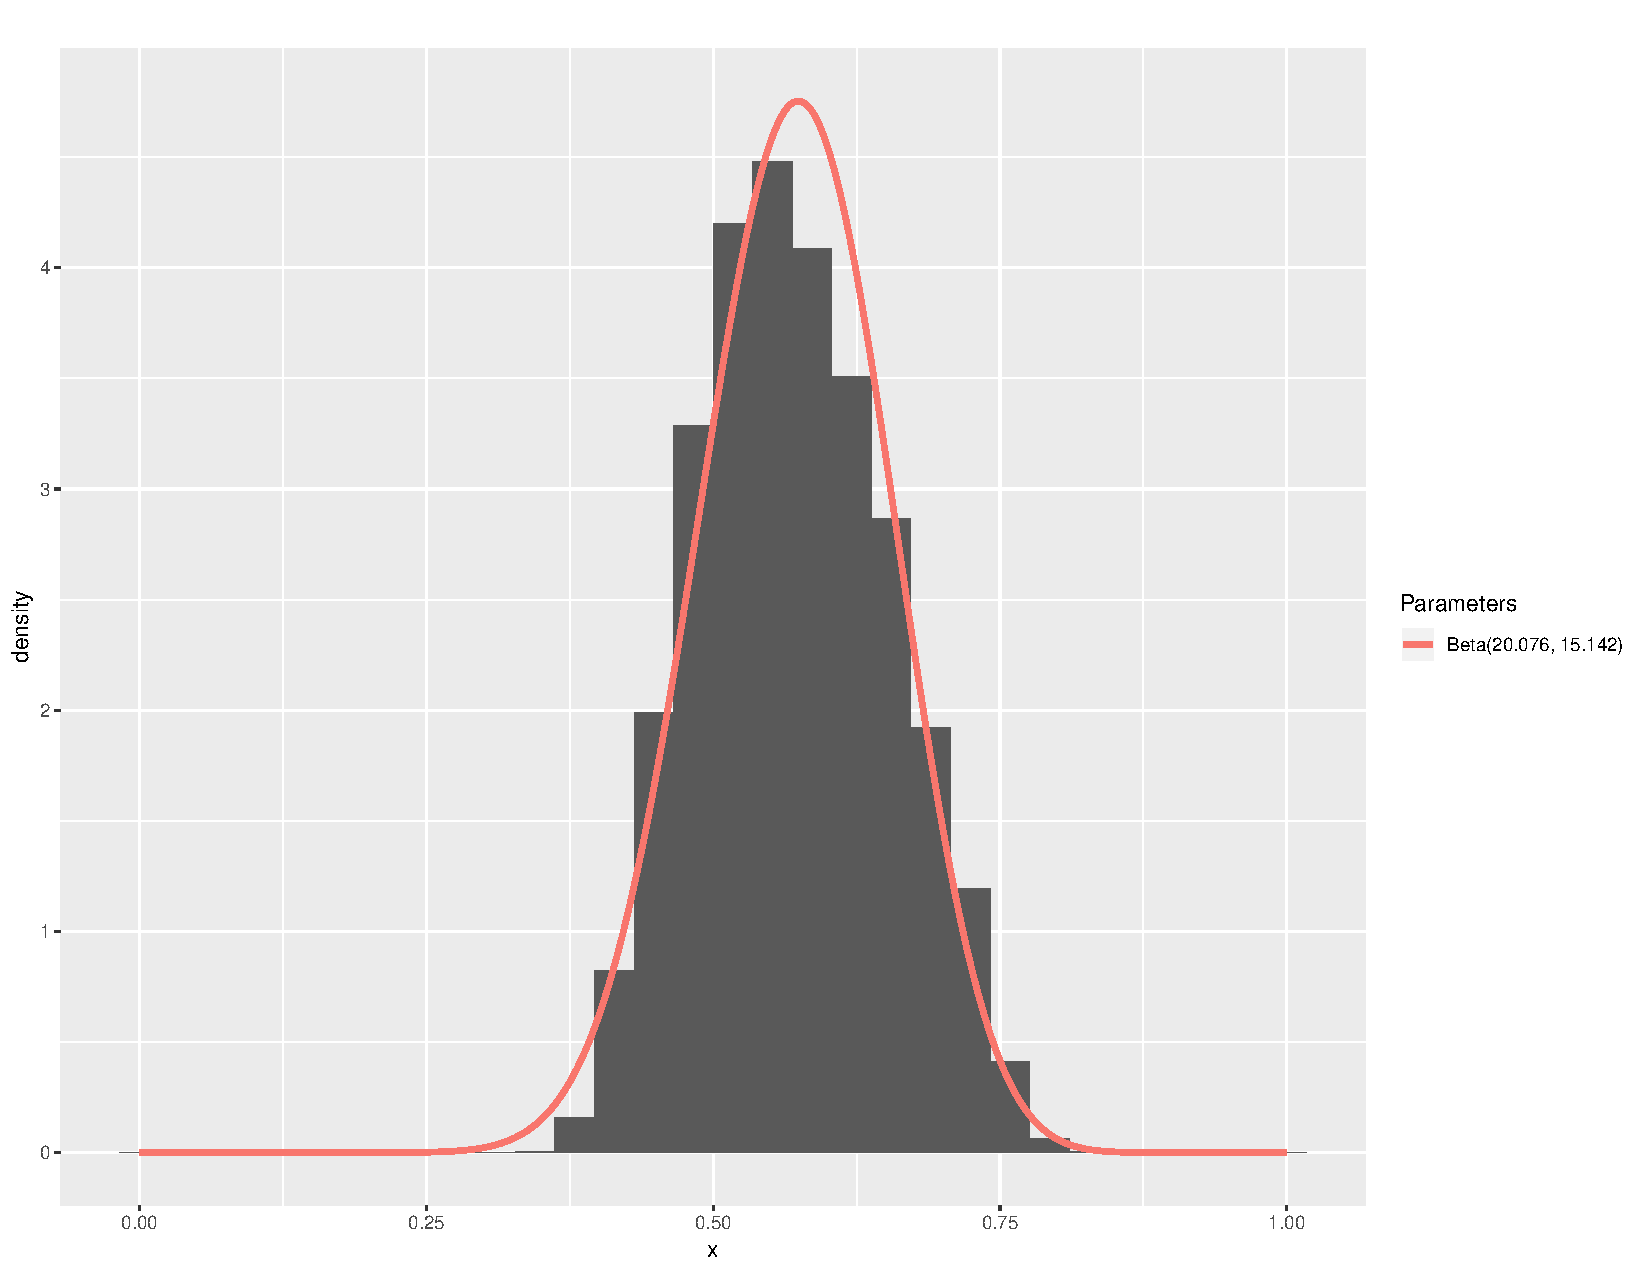
\includegraphics[width=0.8\linewidth]{../../Figures/Report_19_02_27/hist_rv_beta_region1.pdf}
  \caption{Histograma das similaridades dos dados da região 1 a \textit{random volume}}
  \label{fig:hist_beta_rv1}

\end{figure}

\begin{figure}[!h]

  \centering
  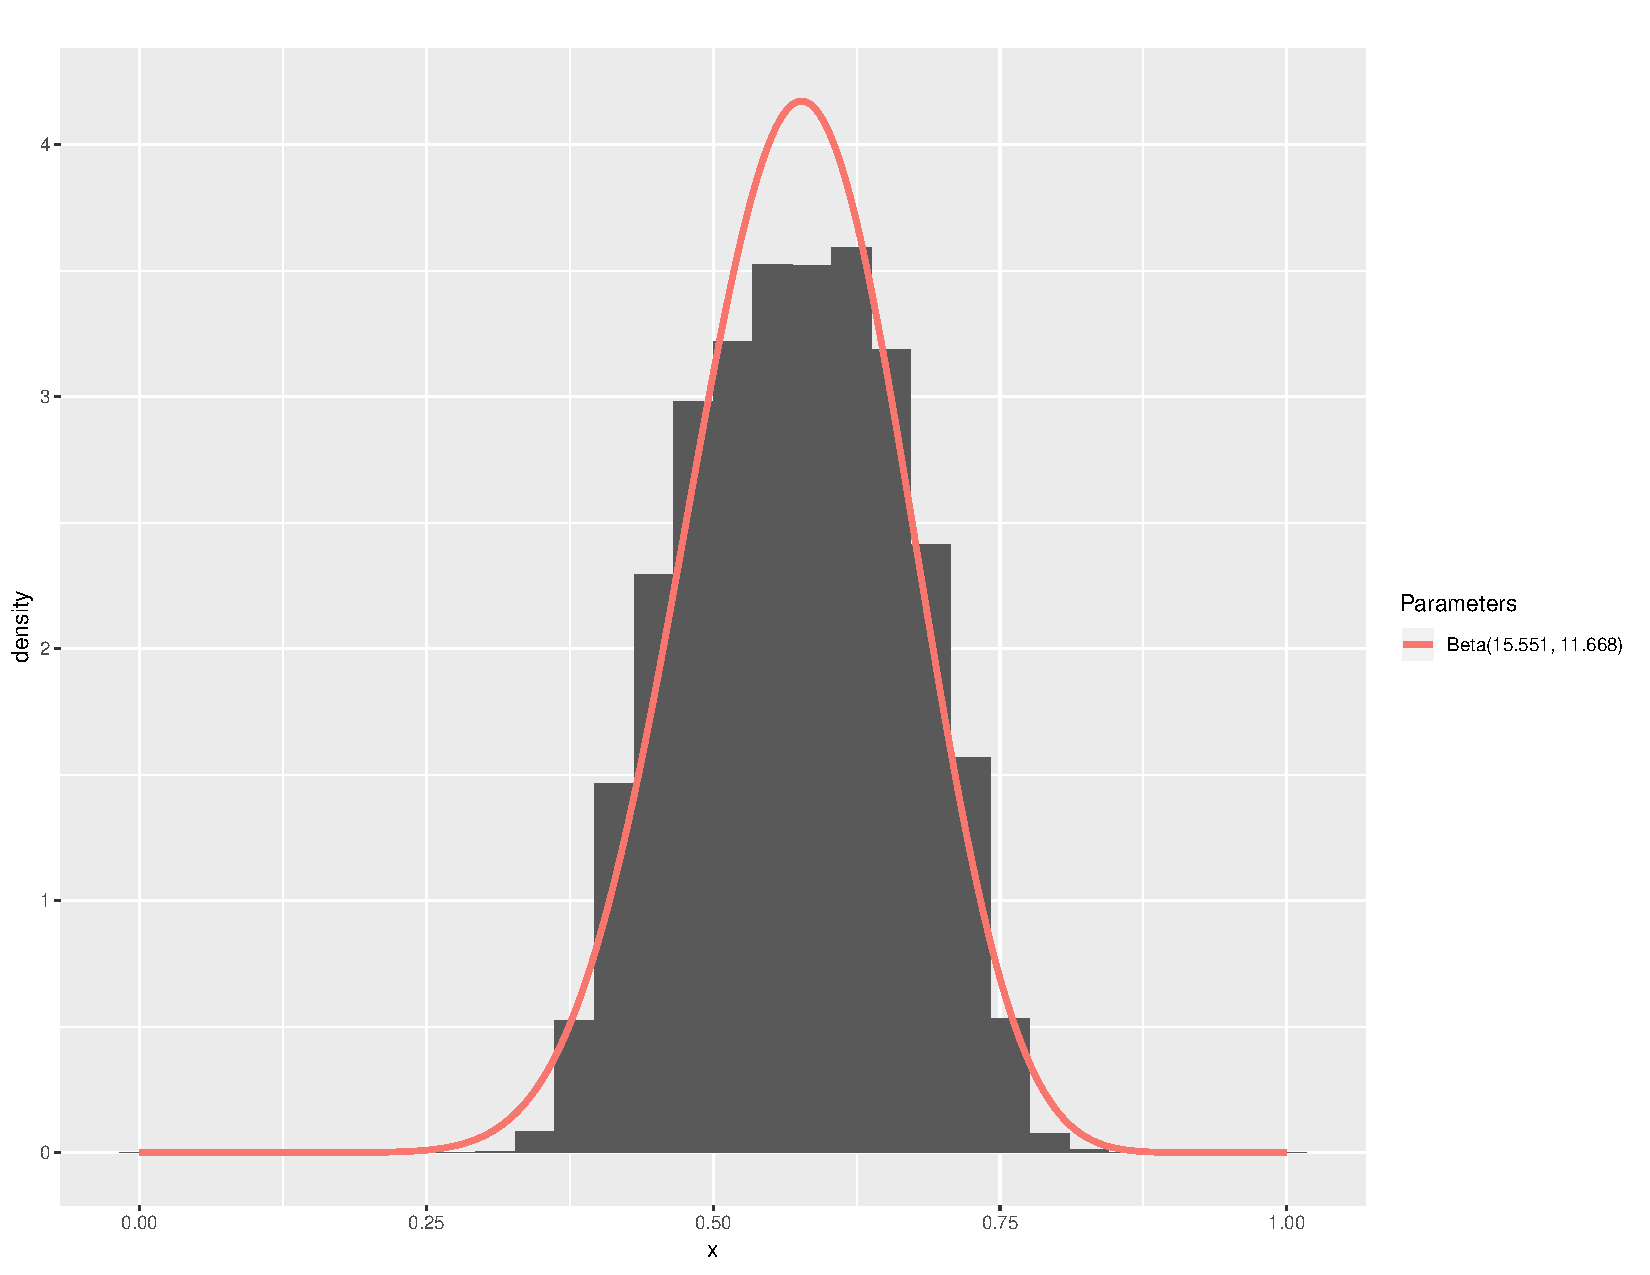
\includegraphics[width=0.8\linewidth]{../../Figures/Report_19_02_27/hist_rv_beta_region2.pdf}
  \caption{Histograma das similaridades dos dados da região 2 a \textit{random volume}}
  \label{fig:hist_beta_rv2}

\end{figure}

\begin{figure}[!h]

  \centering
  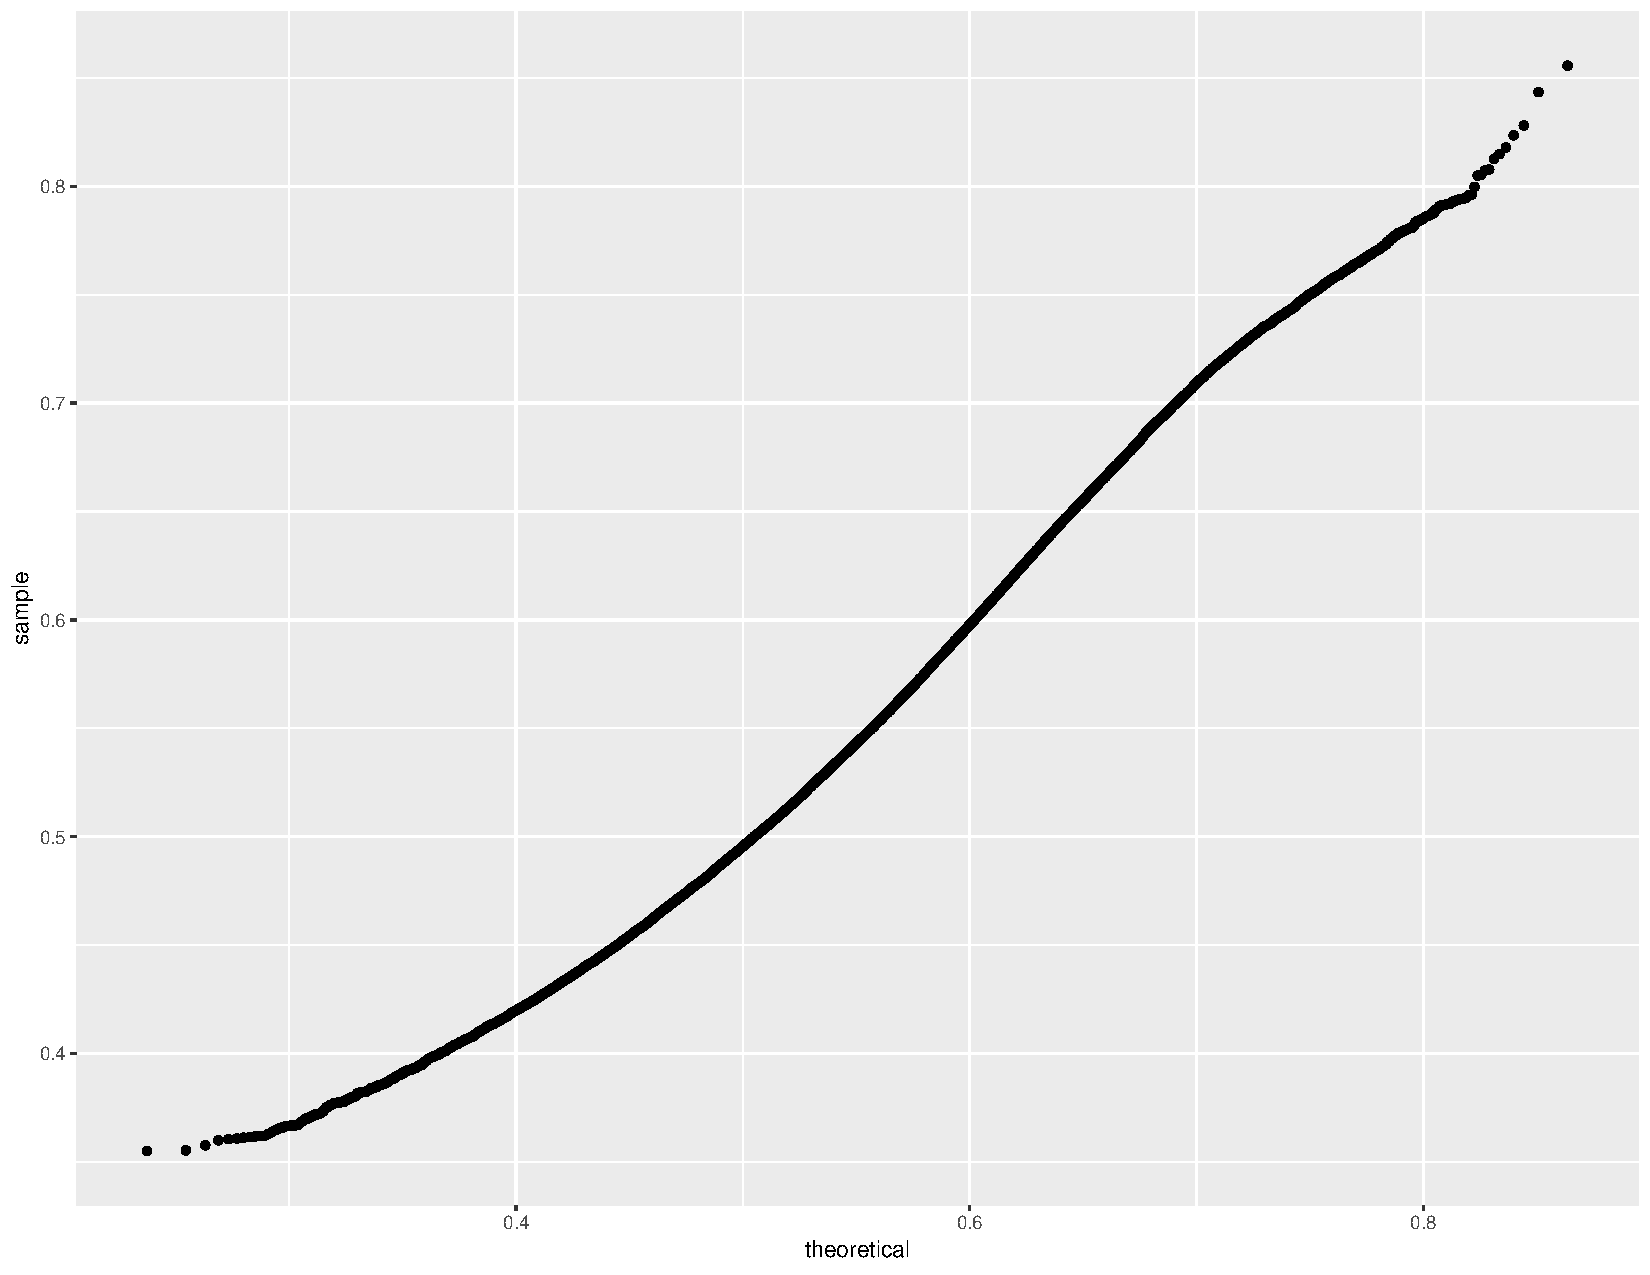
\includegraphics[width=0.8\linewidth]{../../Figures/Report_19_02_27/qqplot_region1.pdf}
  \caption{\textit{qqplot} das similaridades dos dados da região 1 em relação a \textit{random volume} sobre Beta($\alpha$ = 20.076, $\beta$ = 15.142)}
  \label{fig:qqplot_beta_rv1}

\end{figure}

\begin{figure}[!h]

  \centering
  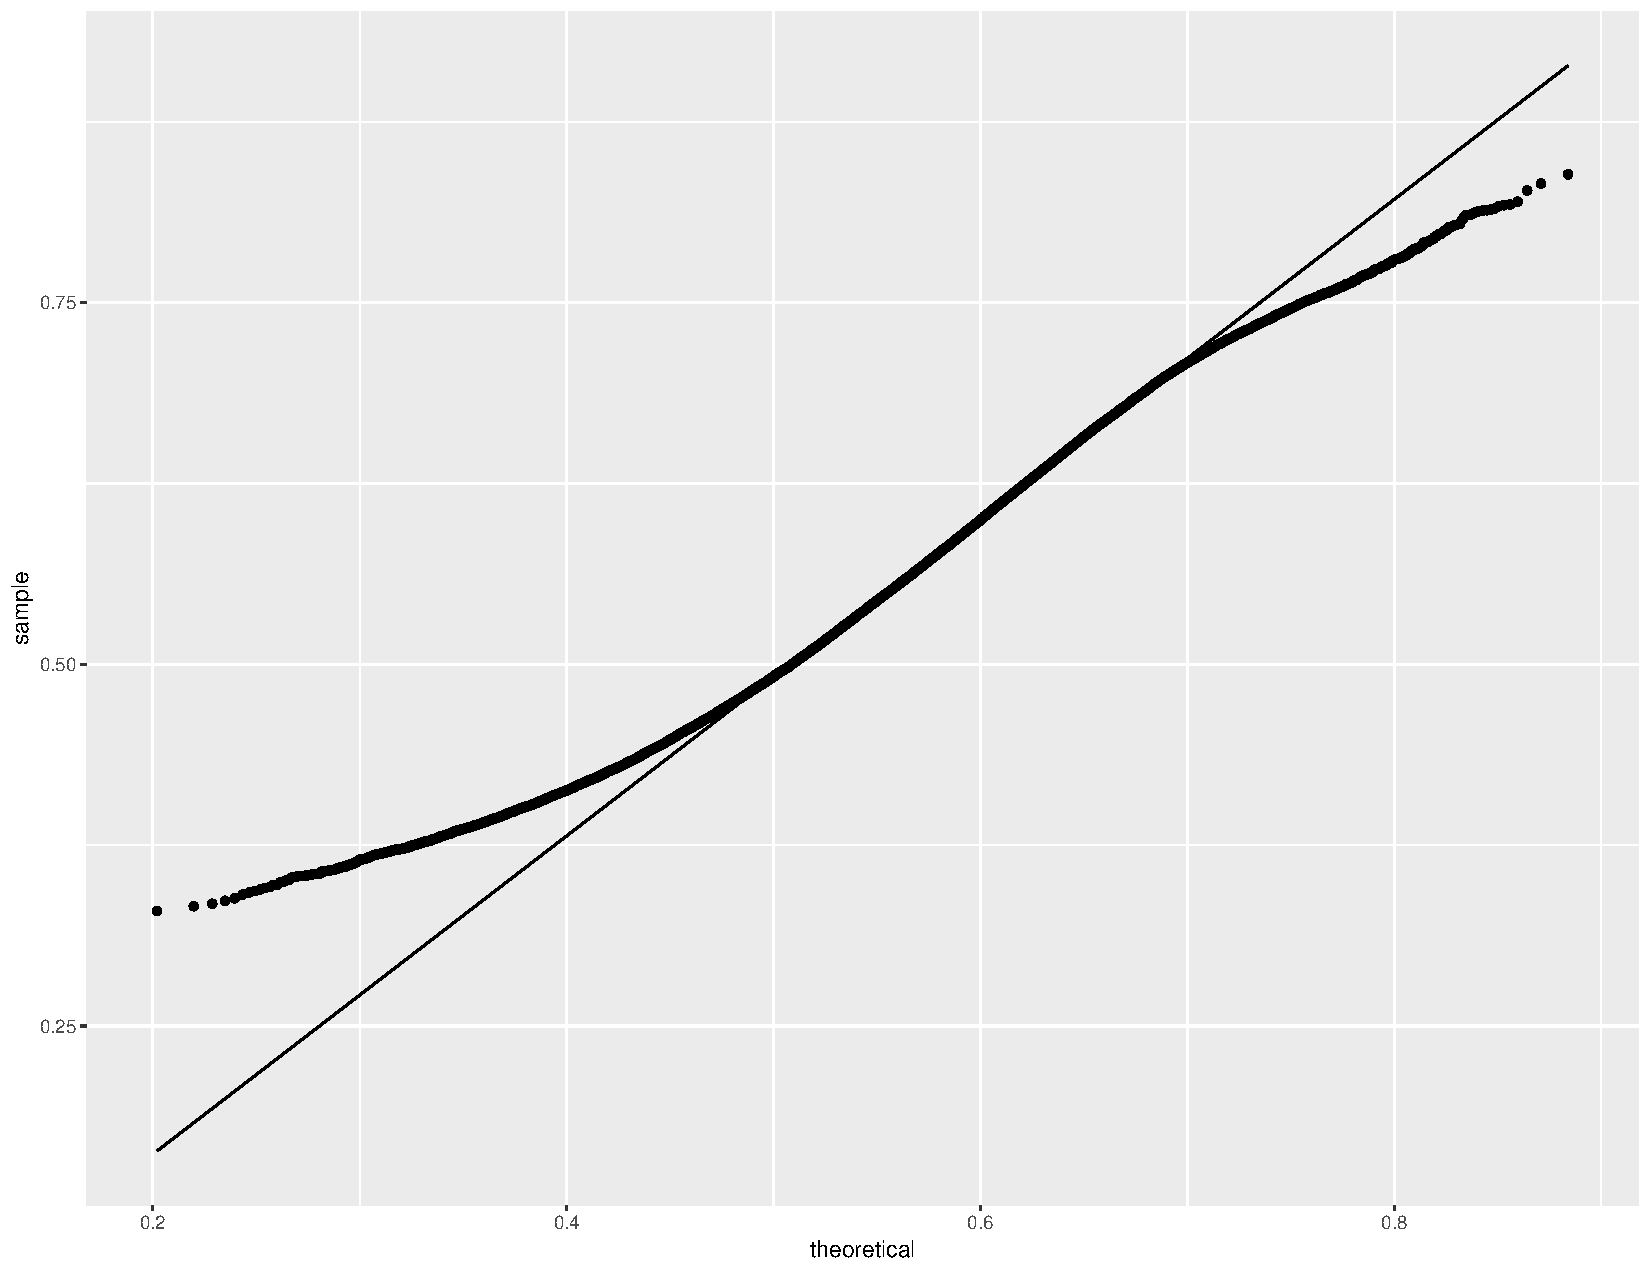
\includegraphics[width=0.8\linewidth]{../../Figures/Report_19_02_27/qqplot_region2.pdf}
  \caption{\textit{qqplot} das similaridades dos dados da região 1 em relação a \textit{random volume} sobre Beta($\alpha$ = 15.822, $\beta$ = 12.182)}
  \label{fig:qqplot_beta_rv2}

\end{figure}

Considerando que a distribuição Beta pode ser reparametrizada em termos de média e variância através das seguintes expressões:

\begin{equation*}
{\alpha} = \frac{(1 - \mu) {\mu}^2 - \mu {\sigma}^2}{{\sigma}^2}
\end{equation*}
\begin{equation*}
{\beta} = \frac{(1 - \mu)[\mu - {\mu}^2 - {\sigma}^2]}{{\sigma}^2}
\end{equation*}
 
Temos que as densidades acima ajustadas em termos de ${\alpha}$ e ${\beta}$ são equivalentes respectivamente à Beta($\mu$ = 0.570, ${\sigma}^2$ = $0.082^2$) e Beta($\mu$ = 0.564, ${\sigma}^2$ = $0.092^2$). Observemos que esses resultados assemelham-se àqueles obtidos anteriormente para regiões de vegetação.

Ao obter-se os \textit{heatmaps} das similaridades em relação a \textit{random volume} das quatro regiões observou-se que as regiões 1 e 2 apresentavam homogeneidade nos mesmos, diferentemente das outras duas, como pode ser observado nas imagens \ref{fig:heat_rv1} a \ref{fig:heat_rv4}. A justificativa é a existência de regiões com diferentes comportamentos de espalhamento, ou seja, diferentes níveis de vegetação.

\begin{figure}[!h]

  \centering
  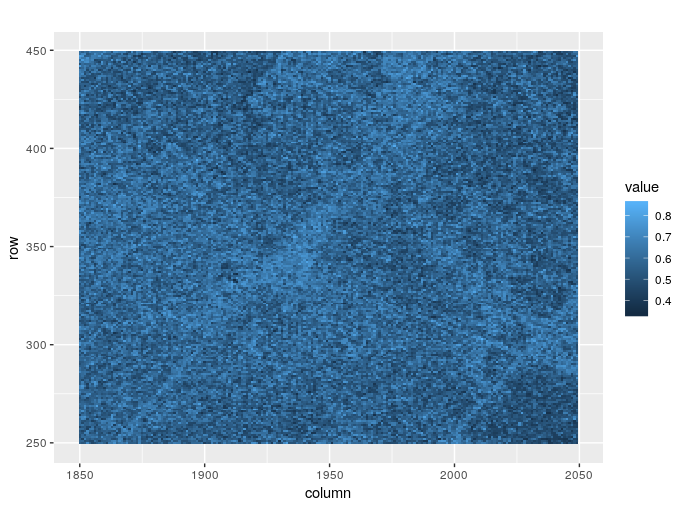
\includegraphics[width=0.8\linewidth]{../../Images/Report_19_02_27/heatmap_rv_region1.png}
  \caption{\textit{heatmap} das similaridades da região 1 em relação a \textit{random volume}}
  \label{fig:heat_rv1}

\end{figure}

\begin{figure}[!h]

  \centering
  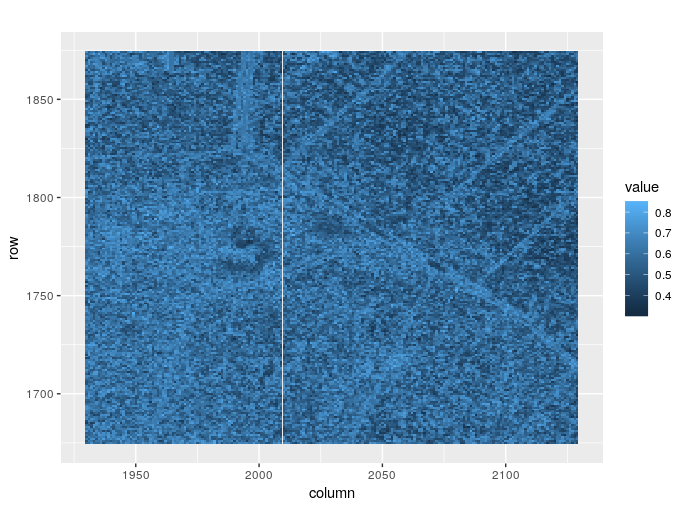
\includegraphics[width=0.8\linewidth]{../../Images/Report_19_02_27/heatmap_rv_region2.png}
  \caption{\textit{heatmap} das similaridades da região 2 em relação a \textit{random volume}}
  \label{fig:heat_rv2}

\end{figure}

\newpage

\begin{figure}[!h]

  \centering
  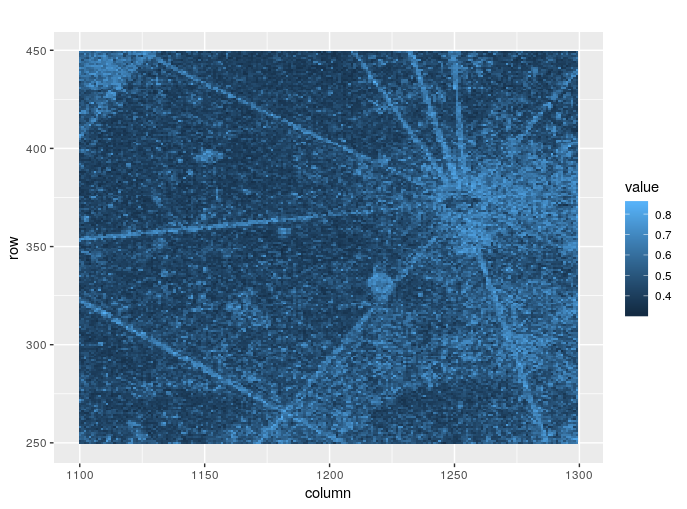
\includegraphics[width=0.8\linewidth]{../../Images/Report_19_02_27/heatmap_rv_region3.png}
  \caption{\textit{heatmap} das similaridades da região 3 em relação a \textit{random volume}}
  \label{fig:heat_rv3}

\end{figure}

\begin{figure}[!h]

  \centering
  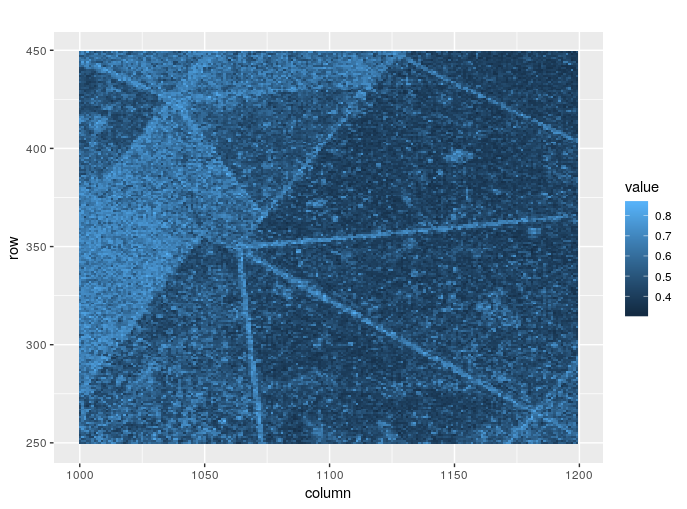
\includegraphics[width=0.8\linewidth]{../../Images/Report_19_02_27/heatmap_rv_region4.png}
  \caption{\textit{heatmap} das similaridades da região 4 em relação a \textit{random volume}}
  \label{fig:heat_rv4}

\end{figure}

\newpage

Nestas duas últimas, ao comparar com as imagens das regiões, observou-se que as subregiões homogêneas e mais escuras no \textit{heatmap} correspondem possivelmente a regiões de solo exposto. Ao analisar uma subregião em cada uma das regiões 3 e 4 com essas características obteve-se os seguintes histogramas e \textit{qqplots}, cujos correspondentes assemelham-se e ajustam-se consideravelmente à função de densidade da distribuição PERT com parâmetros similares.

\begin{figure}[!h]

  \centering
  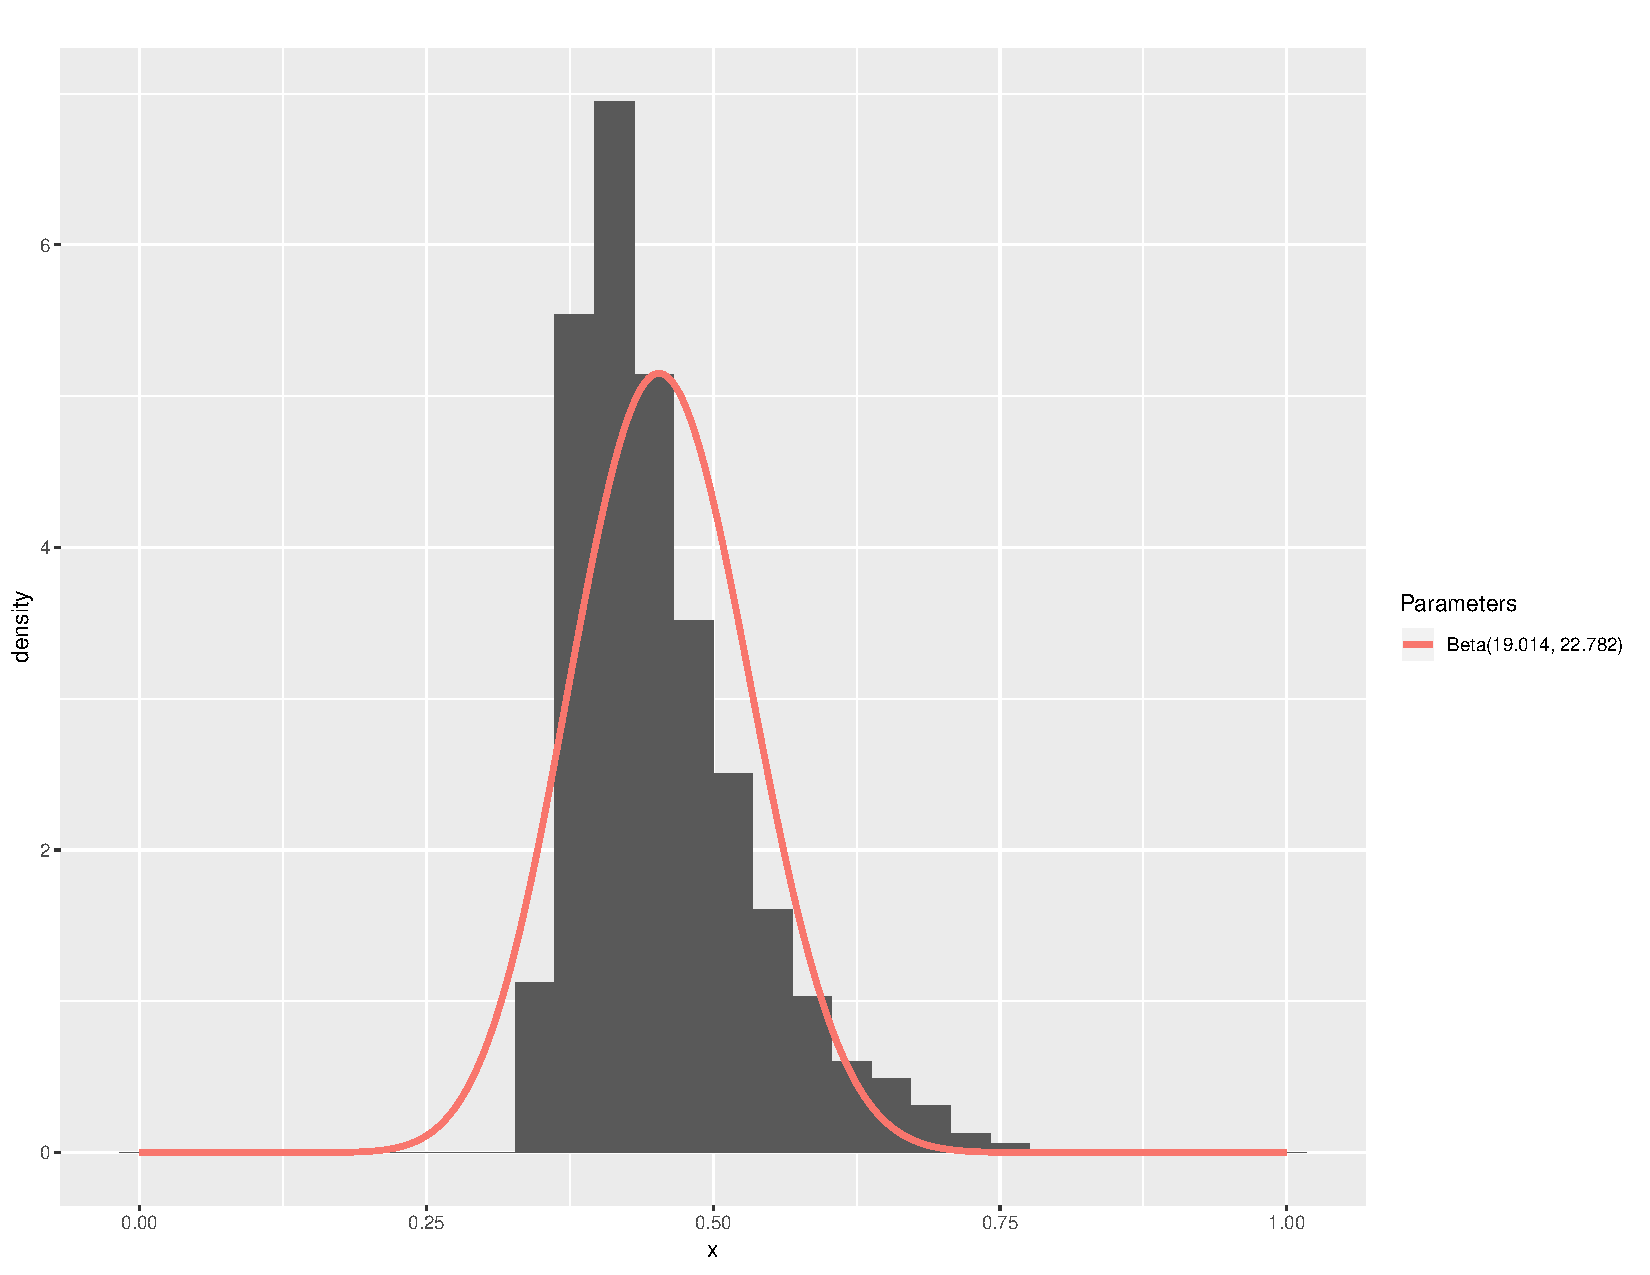
\includegraphics[width=0.8\linewidth]{../../Figures/Report_19_02_27/hist_rv_subregion3.pdf}
  \caption{Histograma das similaridades dos dados de uma subregião de solo exposto da região 3 a \textit{random volume}}
  \label{fig:hist_sub_rv3}

\end{figure}

\begin{figure}[!h]

  \vspace{0.05\linewidth}

  \centering
  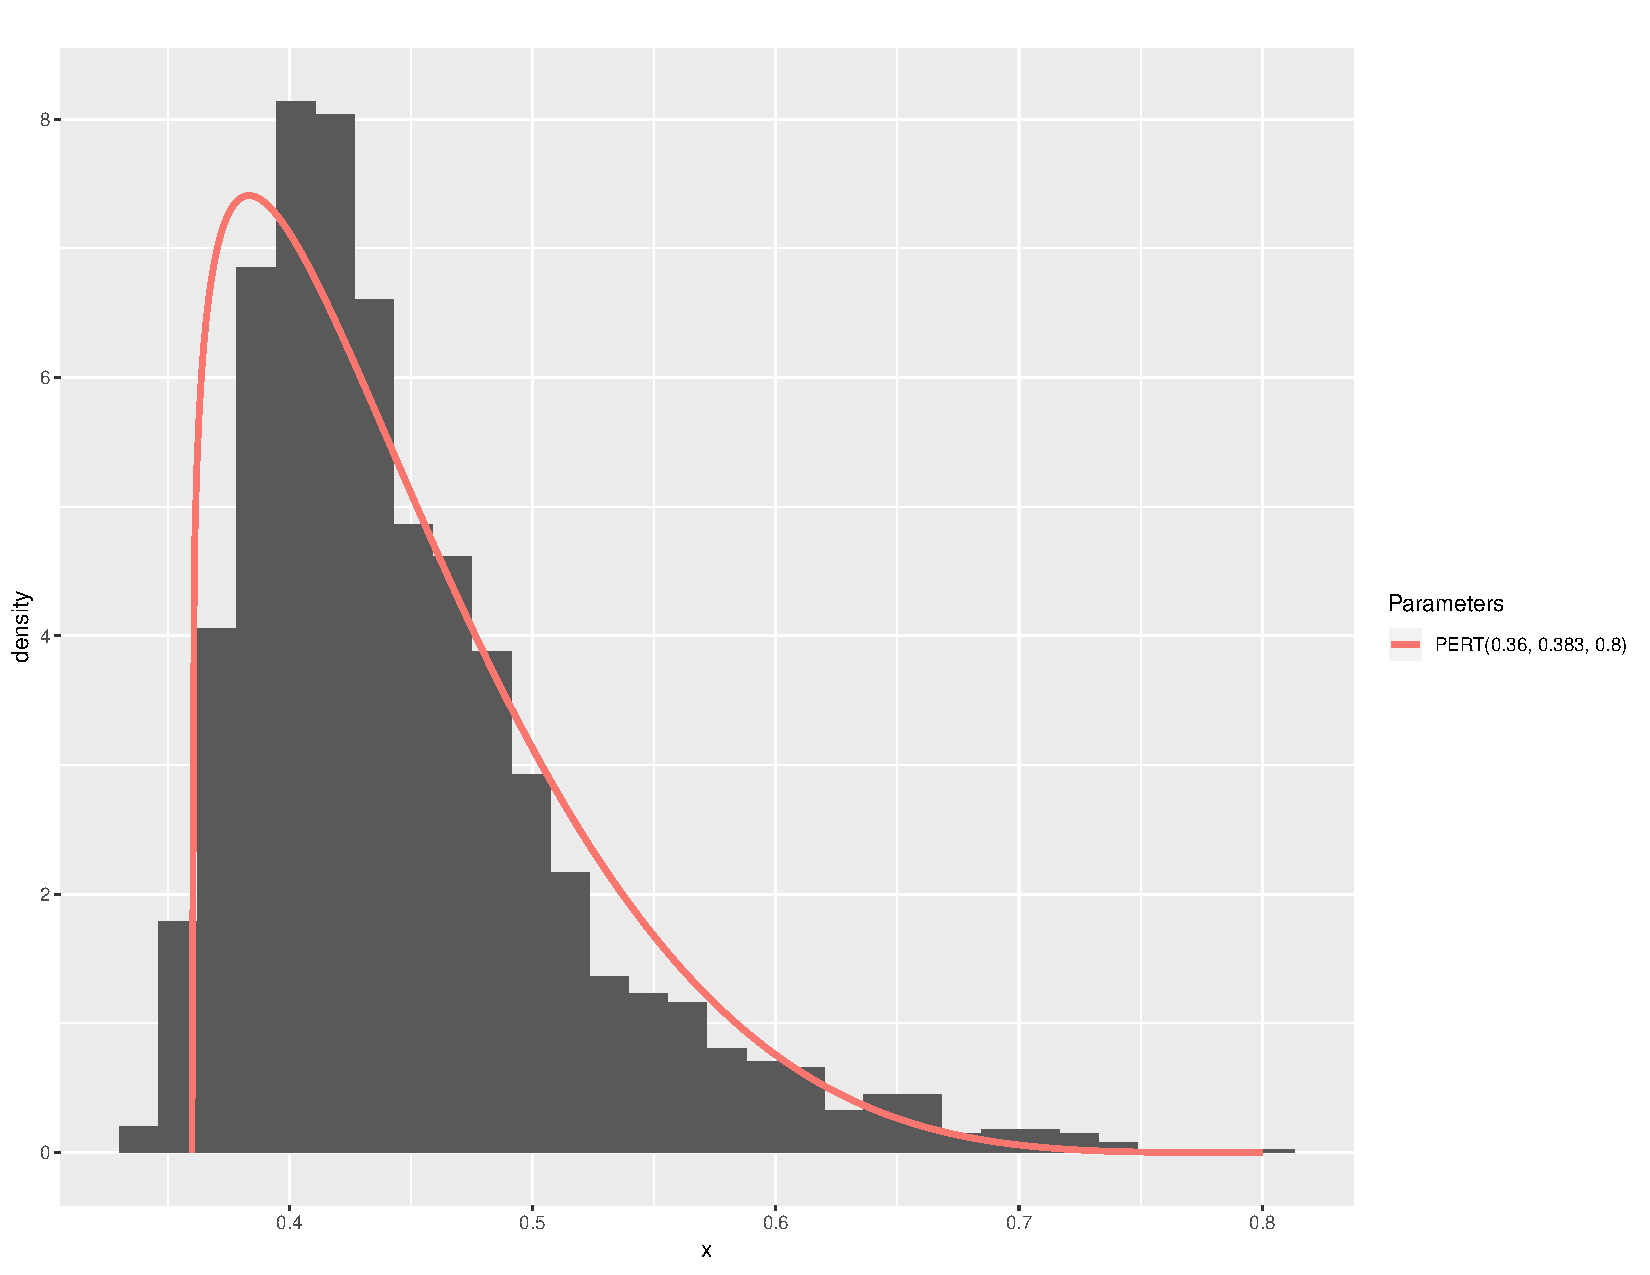
\includegraphics[width=0.8\linewidth]{../../Figures/Report_19_02_27/hist_rv_subregion4.pdf}
  \caption{Histograma das similaridades dos dados de uma subregião de solo exposto da região 4 a \textit{random volume}}
  \label{fig:hist_sub_rv4.1}

\end{figure}

\begin{figure}[!h]

  \vspace{0.1\linewidth}

  \centering
  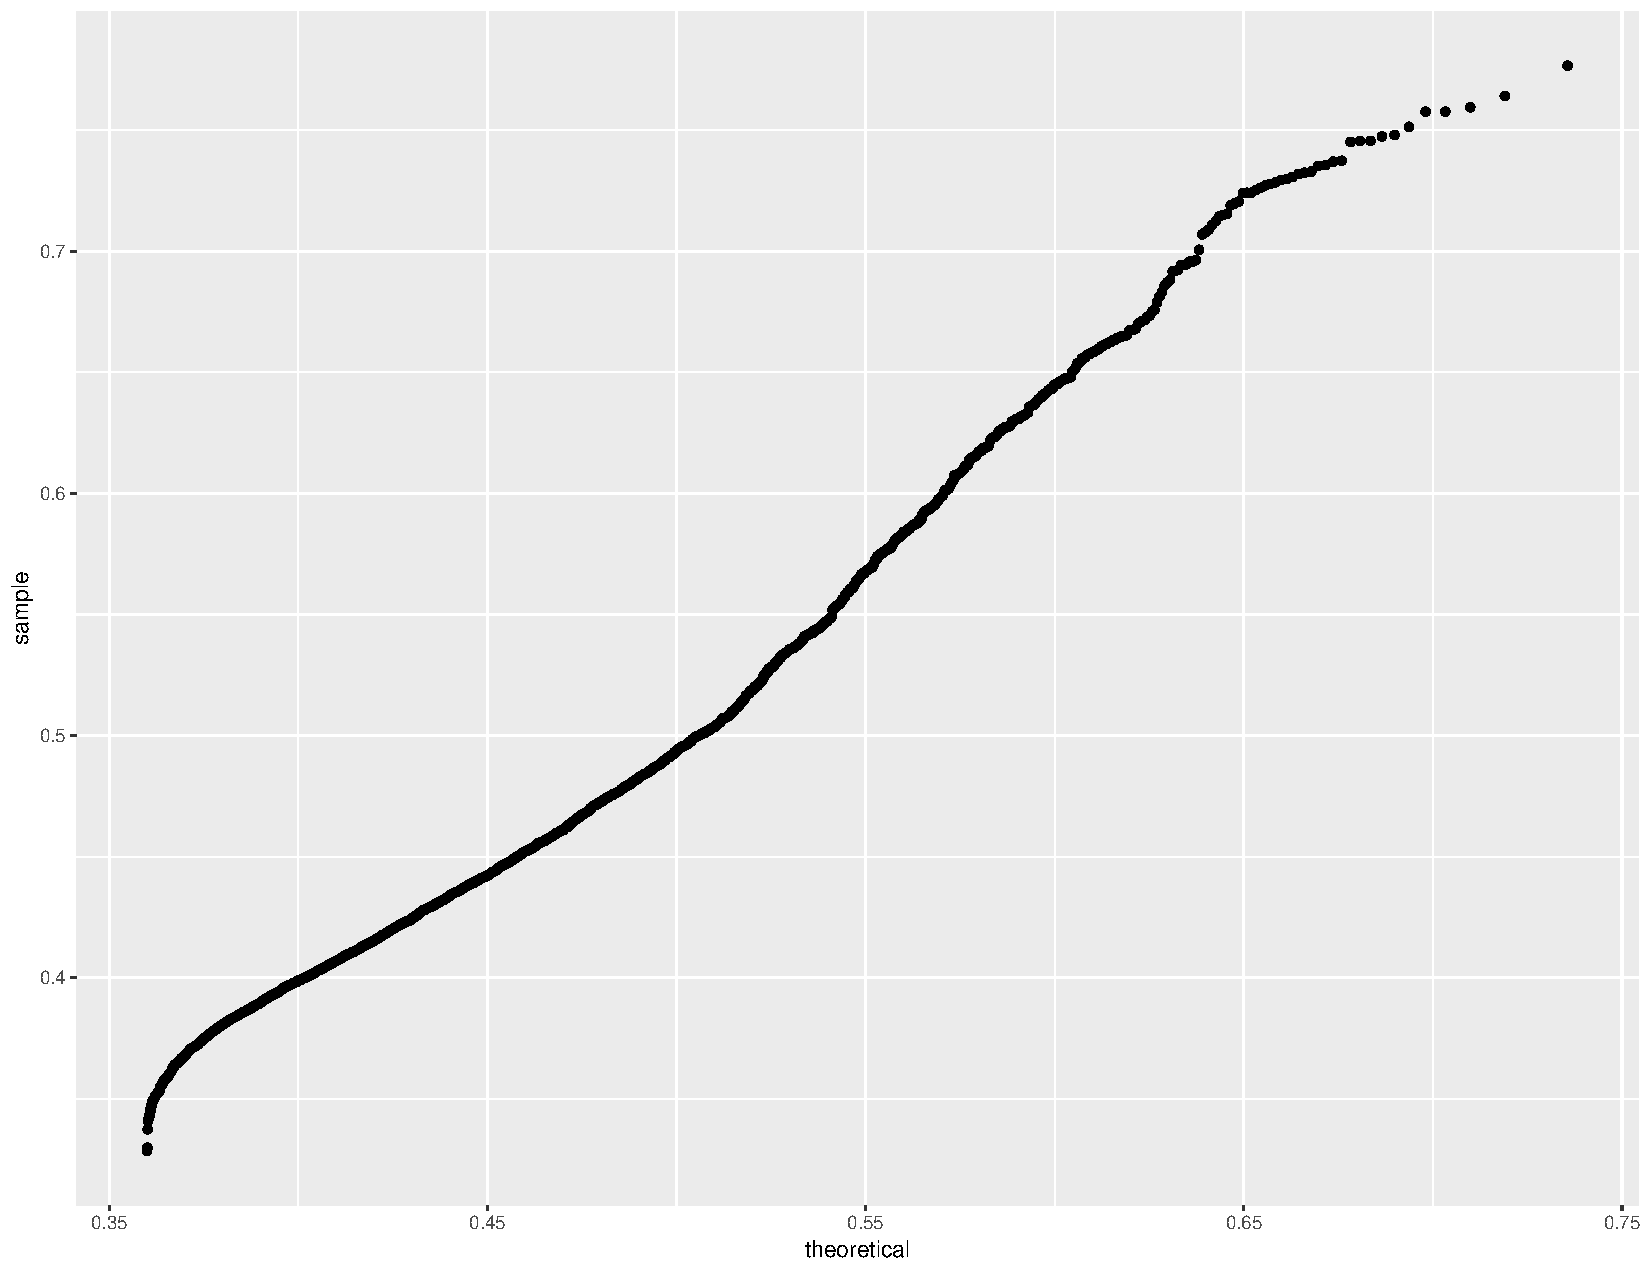
\includegraphics[width=0.8\linewidth]{../../Figures/Report_19_02_27/qqplot_region3.pdf}
  \caption{\textit{qqplot} das similaridades dos dados de uma subregião de solo exposto da região 3 em relação a \textit{random volume} sobre PERT(min = 0.36, mode = 0.38, max = 0.8}
  \label{fig:qqplot_sub_rv3}

\end{figure}

\begin{figure}[!h]

  \centering
  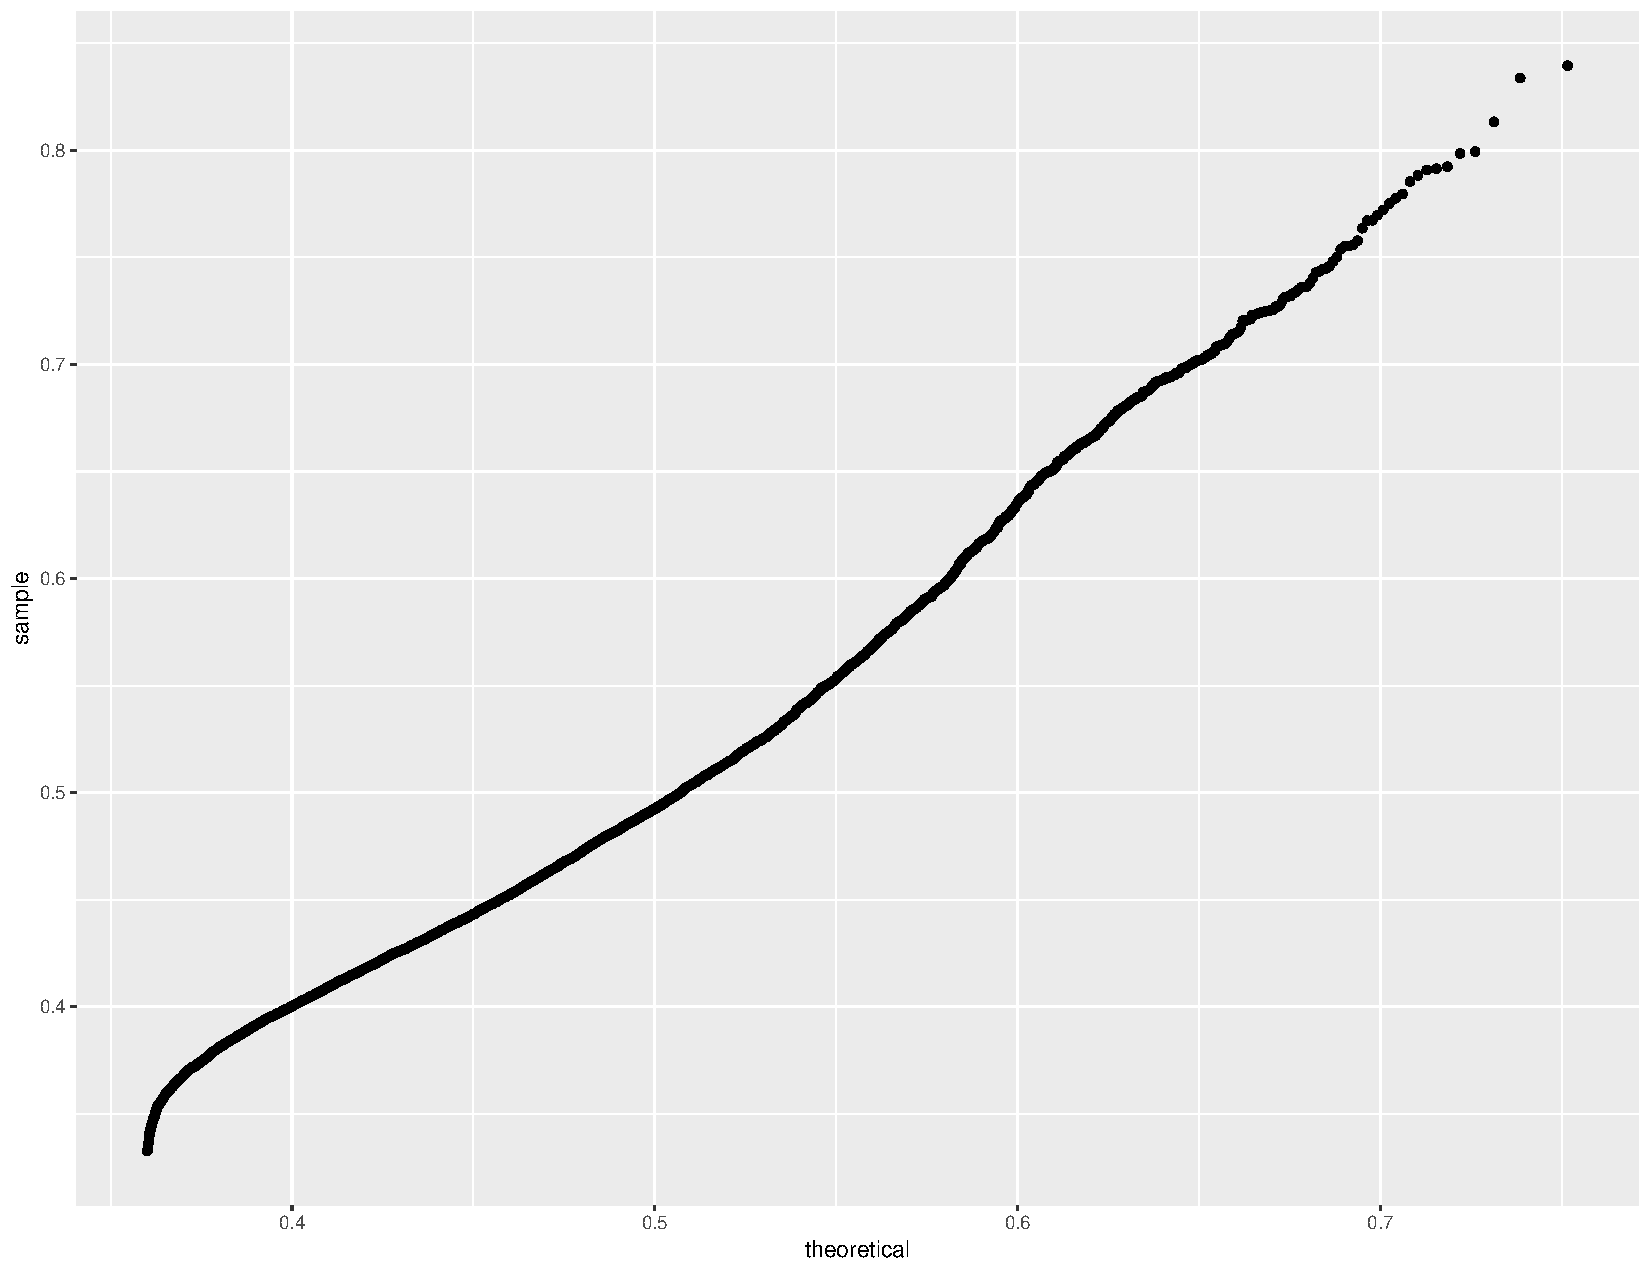
\includegraphics[width=0.75\linewidth]{../../Figures/Report_19_02_27/qqplot_region4.pdf}
  \caption{\textit{qqplot} das similaridades dos dados de uma subregião de solo exposto da região 4 em relação a \textit{random volume} sobre PERT(min = 0.36, mode = 0.398, max = 0.8}
  \label{fig:qqplot_sub_rv4.1}

\end{figure}

\newpage

Ao analisar uma subregião da região 4 que apresenta-se mais clara no \textit{heatmap}, obteve-se o histograma da figura \ref{fig:hist_sub_rv4.2} e o \textit{qqplot} da figura \ref{fig:qqplot_sub_rv4.2}, os quais indicam o ajuste à distribuição Beta. Observemos que o primeiro assemalha-se aos histogramas das regiões 1 e 2. Por isso, supõe-se que essa subregião apresente alguma vegetação. Deve-se salientar que a função de densidade Beta ajustada terá os parâmetros $\mu$ = 0.627 e ${\sigma}^2$ = $0.082^2$ caso seja reparametrizada em função de média e variância.

\begin{figure}[!h]

  \centering
  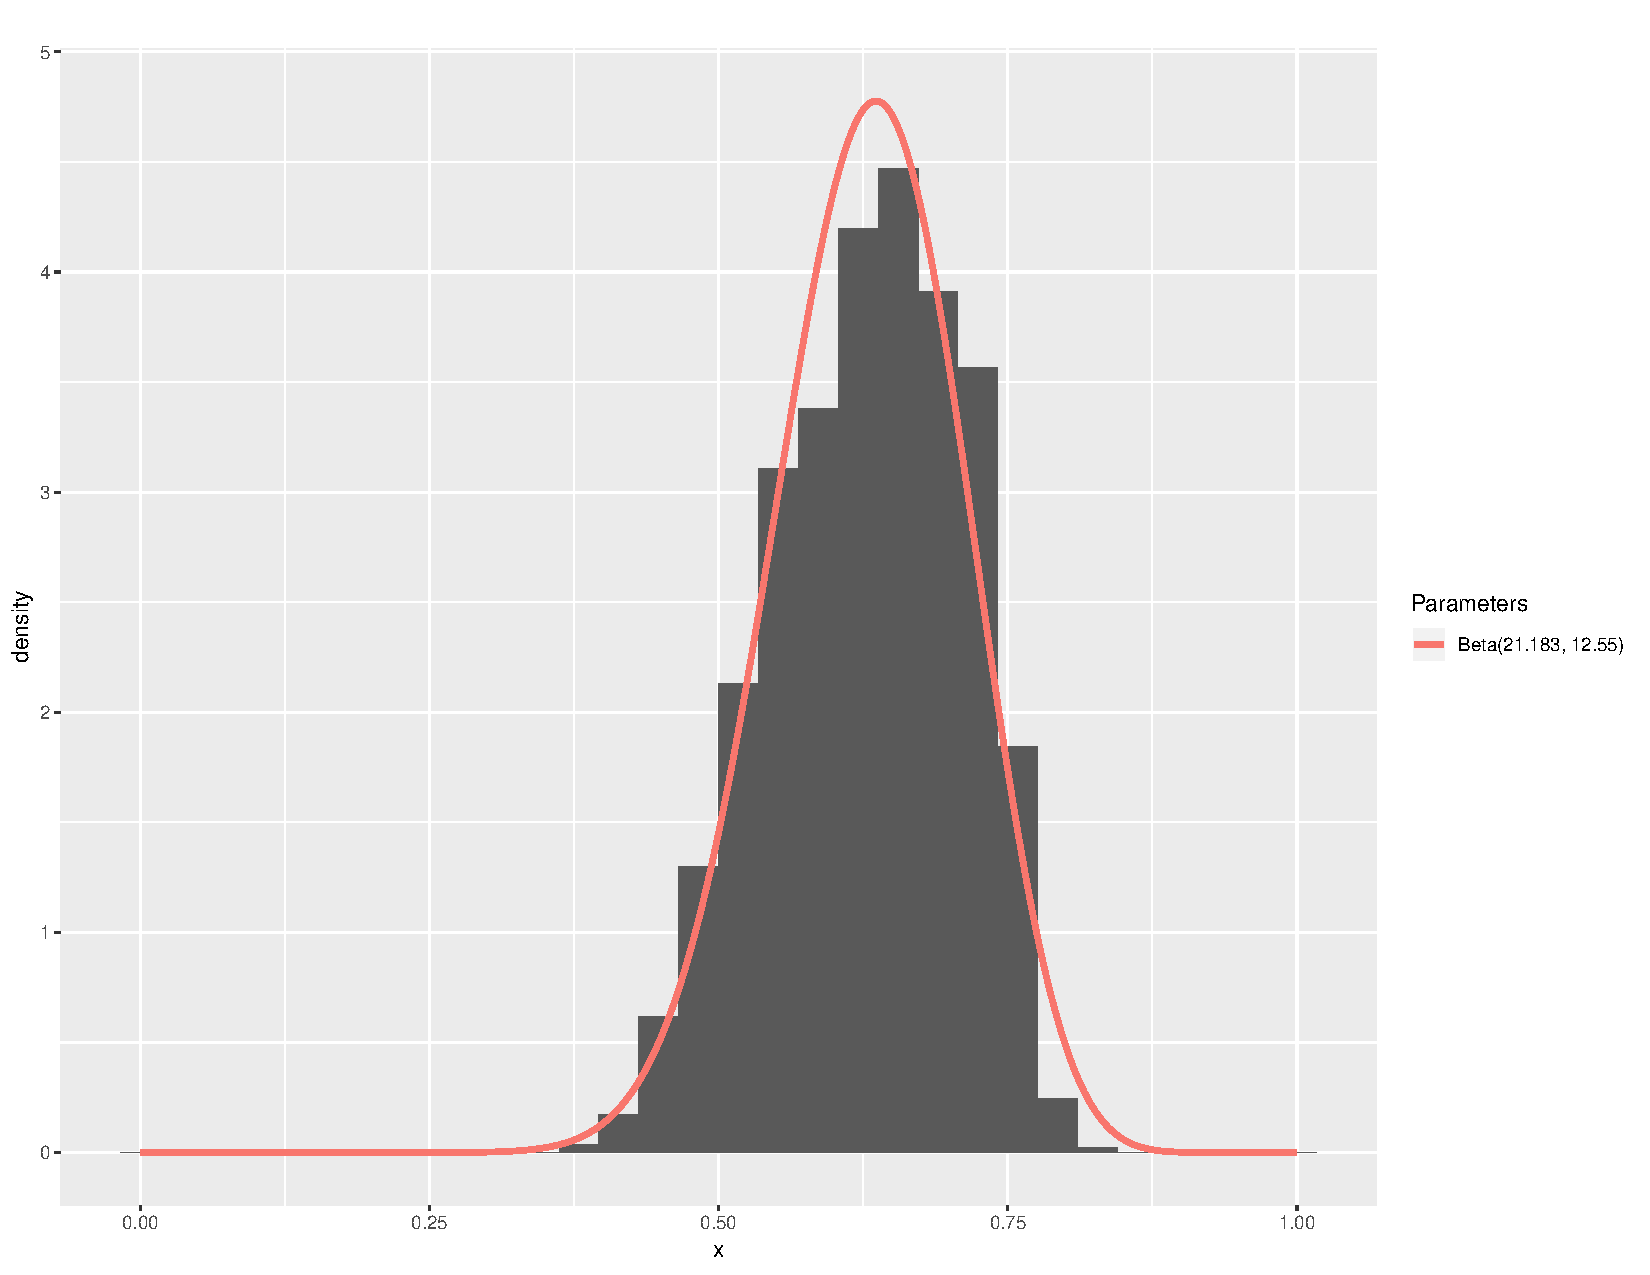
\includegraphics[width=0.75\linewidth]{../../Figures/Report_19_02_27/hist_rv_subregion4_2.pdf}
  \caption{Histograma das similaridades dos dados de uma subregião da região 4 a \textit{random volume}}
  \label{fig:hist_sub_rv4.2}

\end{figure}

\begin{figure}[!h]

  \centering
  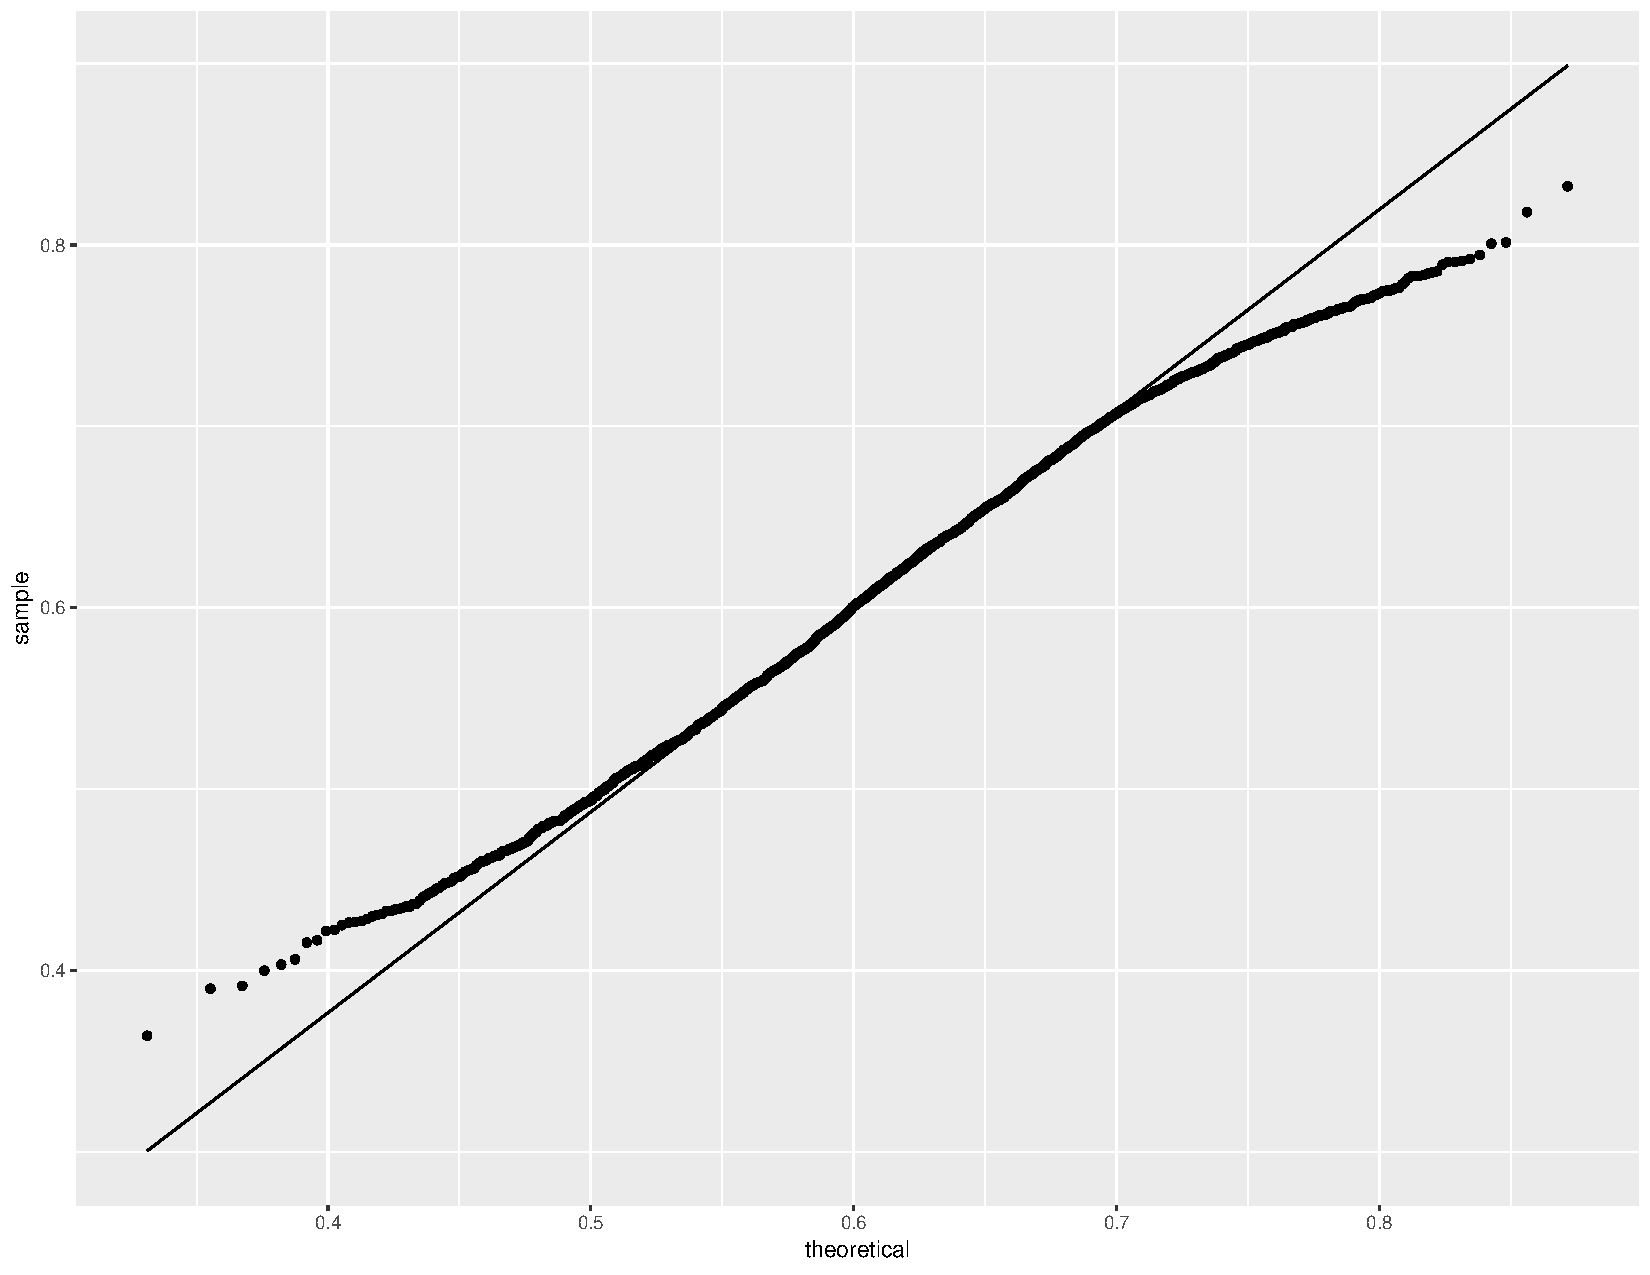
\includegraphics[width=0.8\linewidth]{../../Figures/Report_19_02_27/qqplot_region4_2.pdf}
  \caption{\textit{qqplot} das similaridades dos dados de uma subregião da região 4 em relação a \textit{random volume} sobre Beta($\alpha$ = 21.183, $\beta$ = 12.55)}
  \label{fig:qqplot_sub_rv4.2}

\end{figure}


\section{Teste de aderência}

A fim de validar as afirmações acerca do comportamento estatístico da similaridade do retroespalhador \textit{random volume} em relação aos dados das regiões analisadas, foram realizados testes de aderência Qui-quadrado e Kolmogorov-Smirnov com quatro subregiões de dimensão 20x20 de cada região de análise. Por meio desses testes foram obtidos os p-valores exibidos na tabela \ref{tab:pvalues_table}:

\begin{table}[!ht]
\centering

    \caption{Tabela com p-valores obtidos para os testes de aderência Qui-quadrado (QQ) e Kolmogorov-Smirnov (KS)}
    \label{tab:pvalues_table}     

    \begin{small}
    \begin{tabular}{|l|l|l|l|l|l|l|l|l|}
    \hline
    & \multicolumn{2}{|l|}{\bfseries Subregião 1} & \multicolumn{2}{l|}{\bfseries Subregião 2} & \multicolumn{2}{|l|}{\bfseries Subregião 3} & \multicolumn{2}{l|}{\bfseries Subregião 4} \\
    & {\bfseries QQ} & {\bfseries KS} & {\bfseries QQ} & {\bfseries KS} & {\bfseries QQ} & {\bfseries KS} & {\bfseries QQ} & {\bfseries KS} \\
    \hline
    {\bfseries Região 1} & 0.1754 & 0.2164 & 0.9935 & 0.9767 & 0.3523 & 0.4542 & 0.1729 & 0.345 \\
    {\bfseries Região 2} & 0.1639 & 0.5642 & 0.08146 & 0.3111 & 0.4593 & 0.3722 & 0.9475 & 0.8463 \\
    {\bfseries Região 3} & 0.01799 & 0.4191 & 0.06297 & 0.5063 & 0.0004998 & 0.06616 & 0.0004998 & 0.002288 \\
    {\bfseries Região 4} & 0.0004998 & 0.0584 & 0.0004998 & 0.0181 & 0.0004998 & 0.2903 & 0.7406 & 0.5302 \\
    \hline
    \end{tabular} 
    \end{small} 
\end{table}

Acerca do teste Qui-quadrado, deve-se ressaltar que o intervalo de similaridades observadas foi dividido em subintervalos de comprimento 0.05 para a realização do teste, excetuanto quando ocorreu a união desses subintervalos devido o número de observações em um subintervalo ter sido inferior a 5 ou a probabilidade do mesmo segundo a distribuição ser igual a 0.

Analisando a tabela \ref{tab:pvalues_table} observa-se que apesar obter-se altos p-valores para algumas amostras, o que intensifica a suposição de que as similaridades obedecem às distribuições analisadas, há também p-valores muito baixos. Isto possivelmente justifica-se na qualidade das amostras que pode ser atestada devido a falta de dados de campo.

\section{Histogramas das similaridades em relação aos demais retroespalhadores elementares}

As figuras \ref{fig:hists1} à \ref{fig:hists4} apresentam respectivamente os histogramas das similaridades dos dados (não filtrados) das regiões 1 à 4 aos retroespalhadores prototípicos. Observemos que os histogramas das regiões 1 e 2 assemelham-se assim como os das regiões 3 e 4, contudo os das duas primeiras diferem daquelas pertencentes às duas últimas. Deve ser observado também que alguns histogramas refrentes à região 2 apresentam um caráter bimodal, isto possivelmente ocorre devido à presença de dados de outras populações.

\begin{figure}[!h]

  \centering
  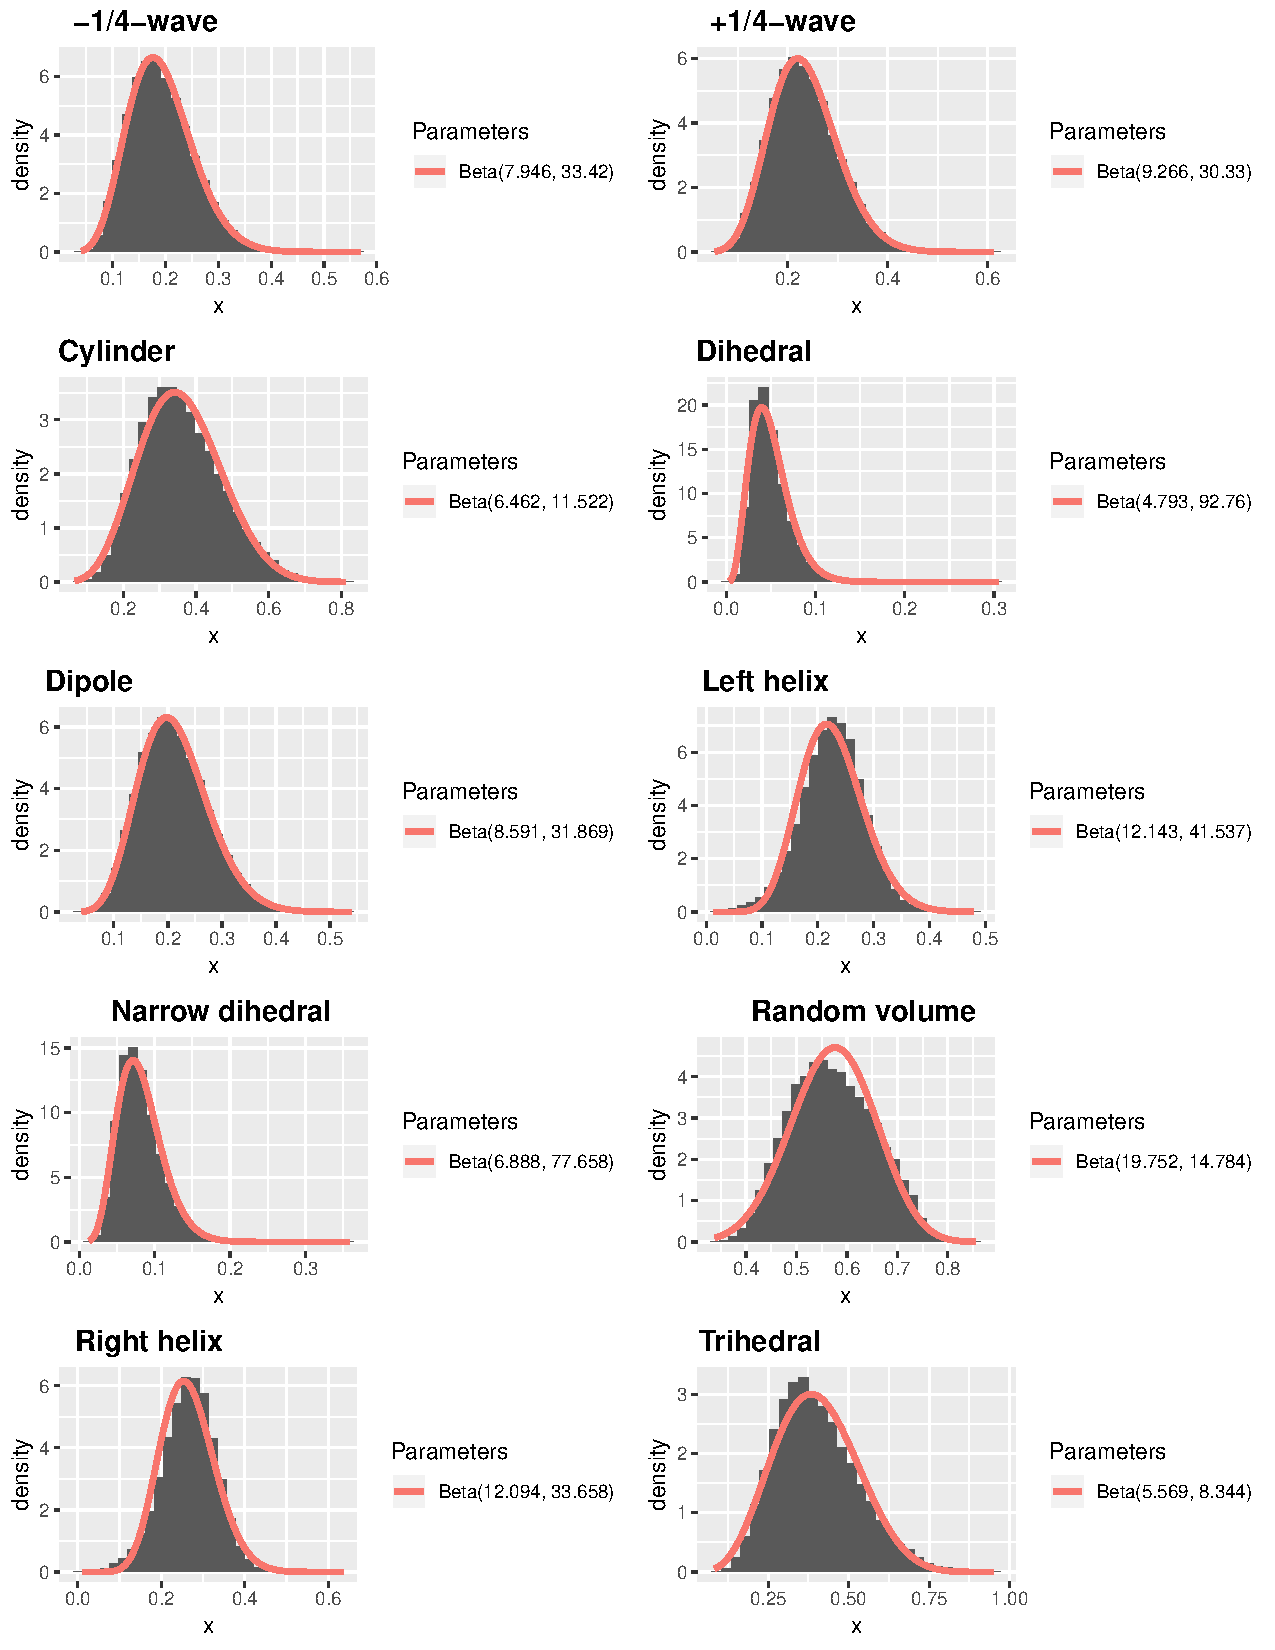
\includegraphics[width = 0.75\linewidth]{../../Figures/Report_19_02_27/region1_plots.pdf}
  \caption{Histogramas referentes às similaridades dos dados da região 1 em relação aos retroespalhadores elementares}
  \label{fig:hists1}

\end{figure}

\newpage

\begin{figure}[!h]
  \vspace{0.1\linewidth}
  \centering
  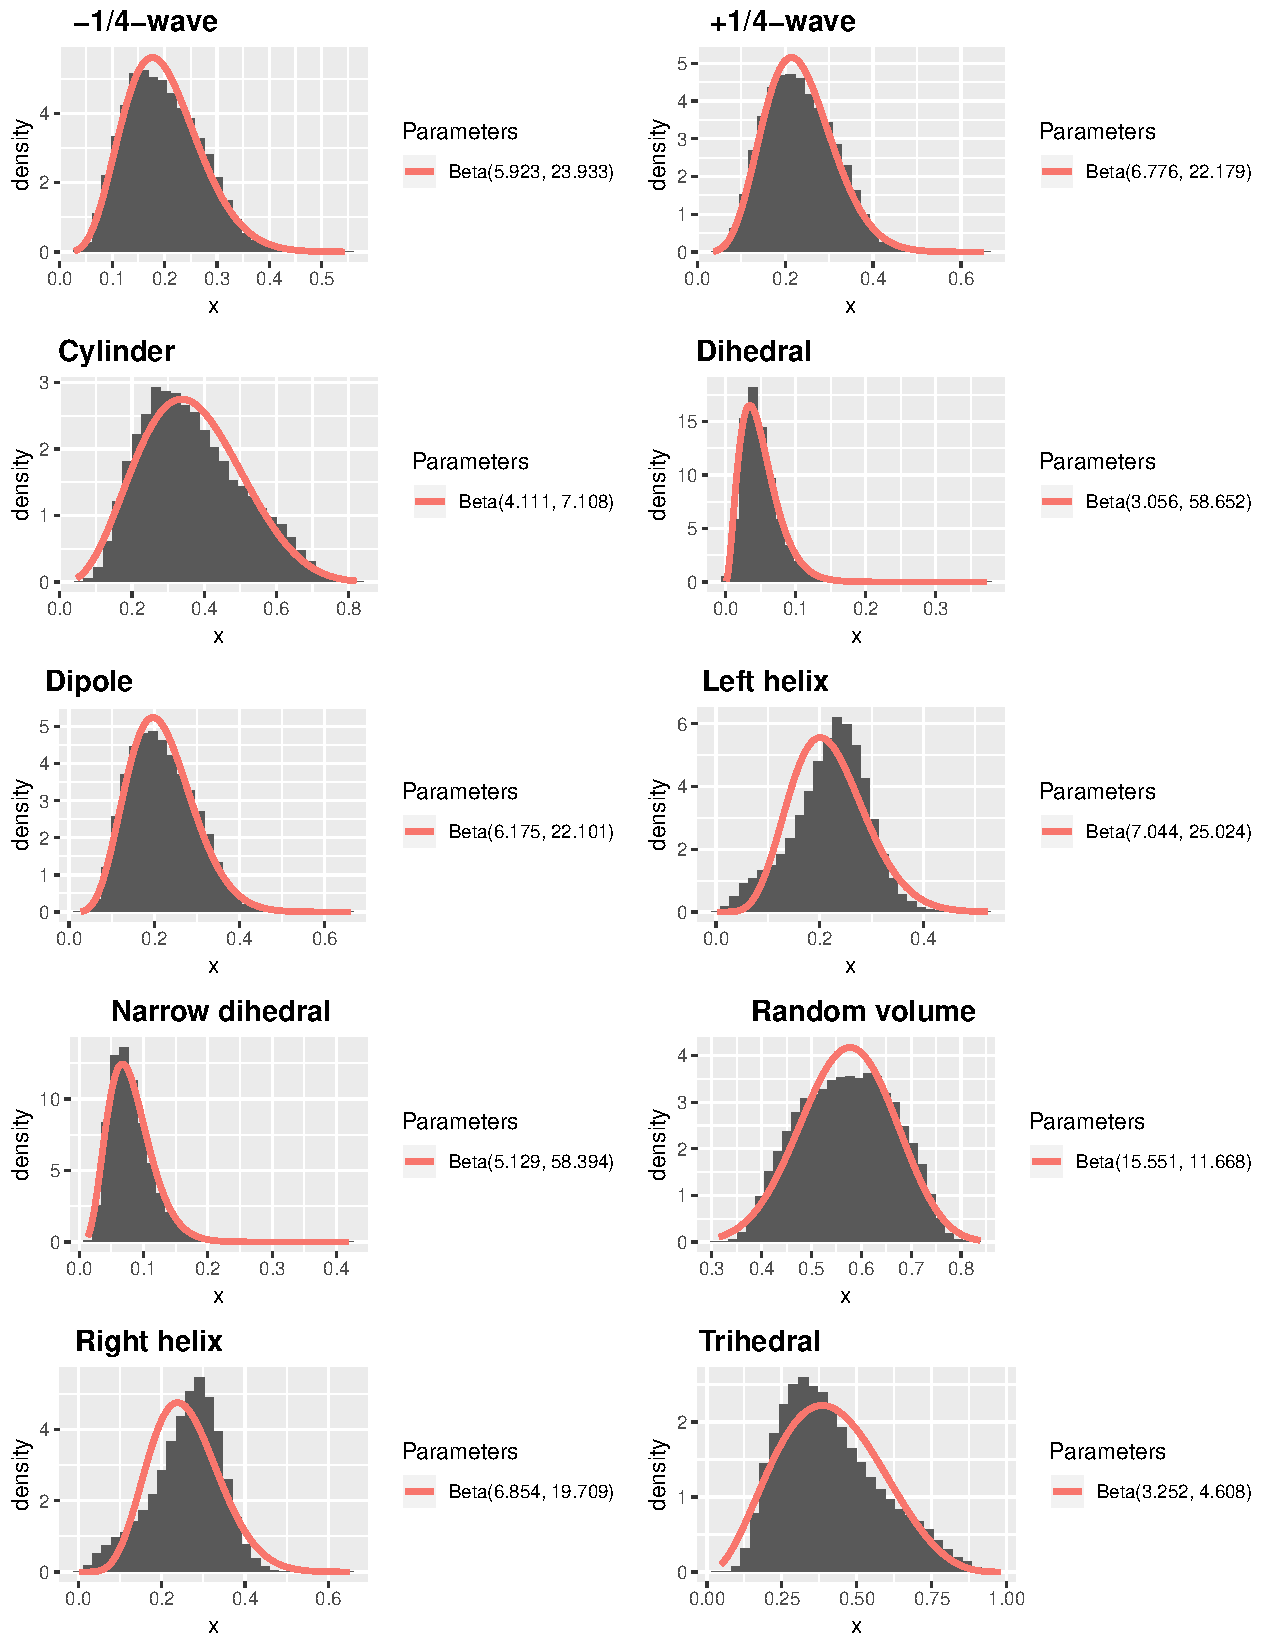
\includegraphics[width = 0.8\linewidth]{../../Figures/Report_19_02_27/region2_plots.pdf}
  \caption{Histogramas referentes às similaridades dos dados da região 2 em relação aos retroespalhadores elementares}
  \label{fig:hists2}

\end{figure}

\newpage

\begin{figure}[!h]
  \vspace{0.1\linewidth}
  \centering
  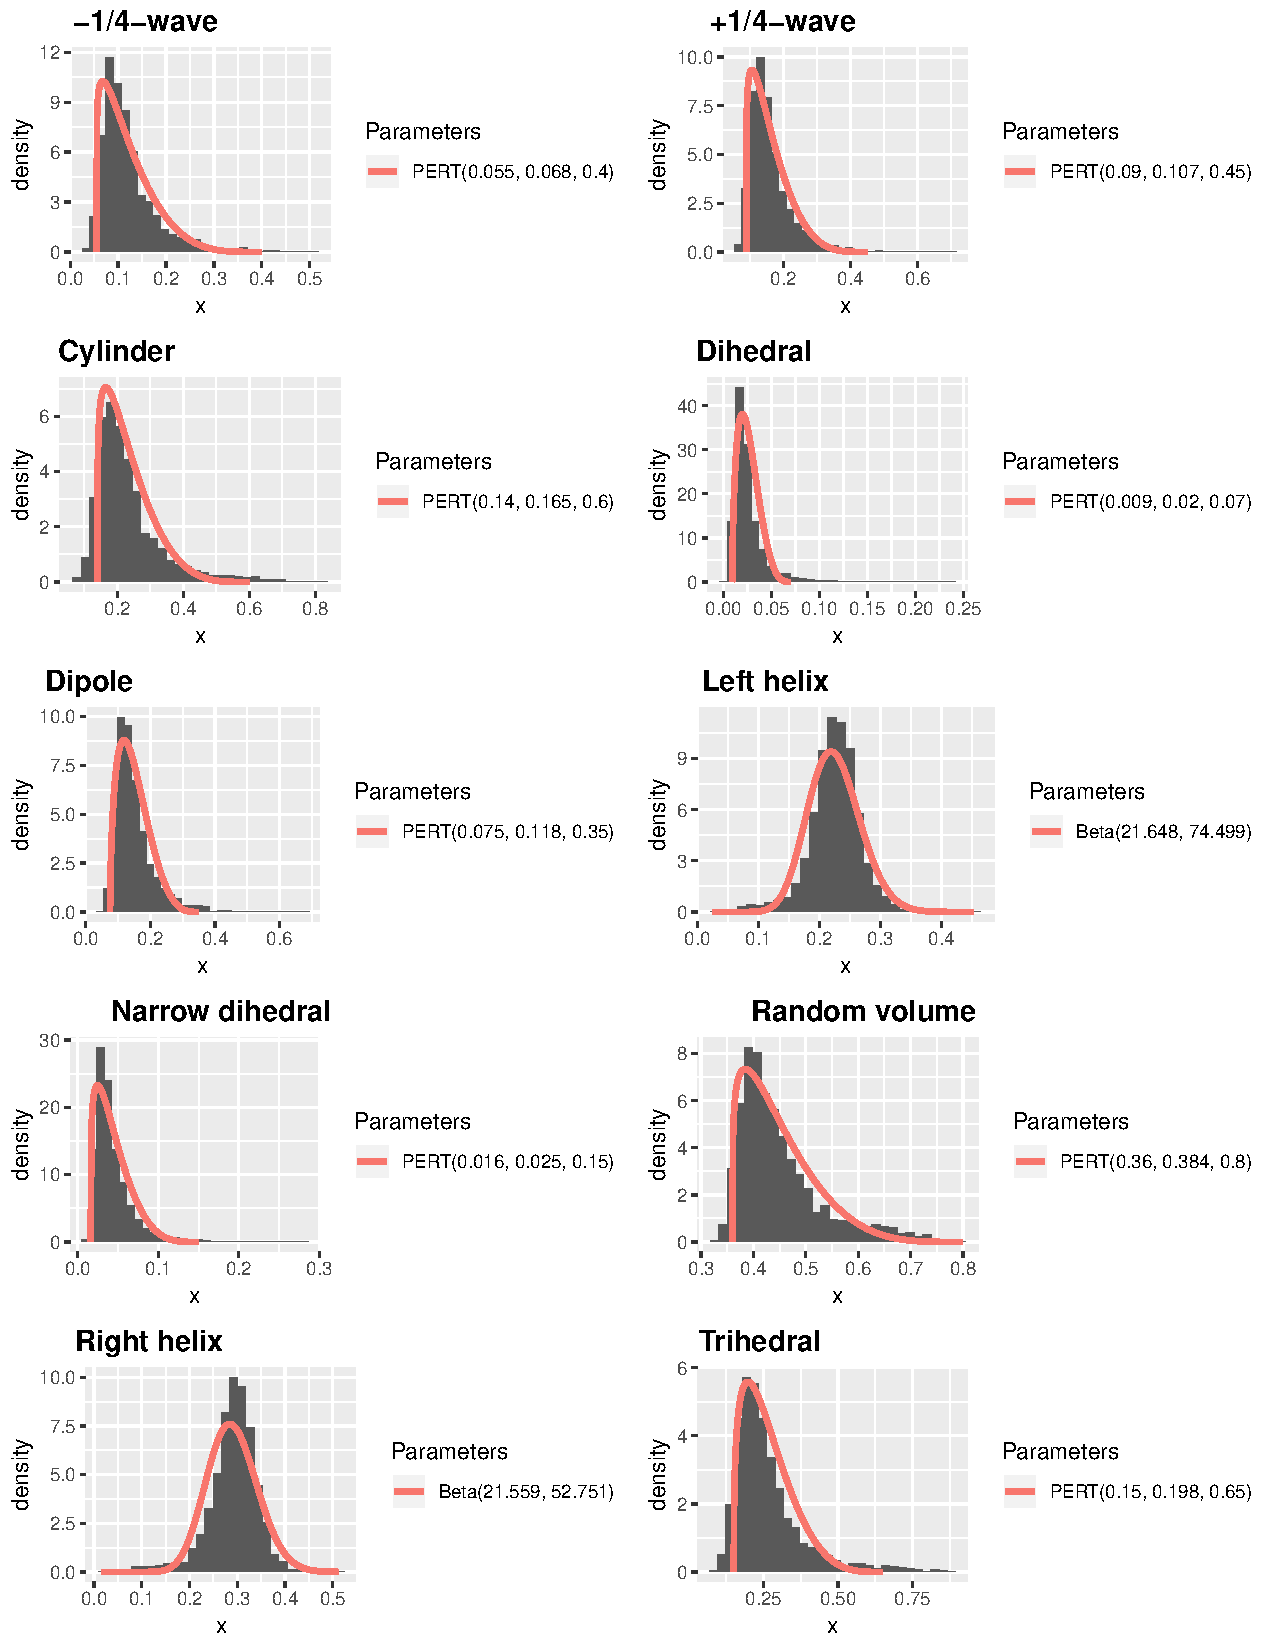
\includegraphics[width = 0.8\linewidth]{../../Figures/Report_19_02_27/region3_plots.pdf}
  \caption{Histogramas referentes às similaridades dos dados da região 3 em relação aos retroespalhadores elementares}
  \label{fig:hists3}

\end{figure}

\newpage

\begin{figure}[!h]

  \centering
  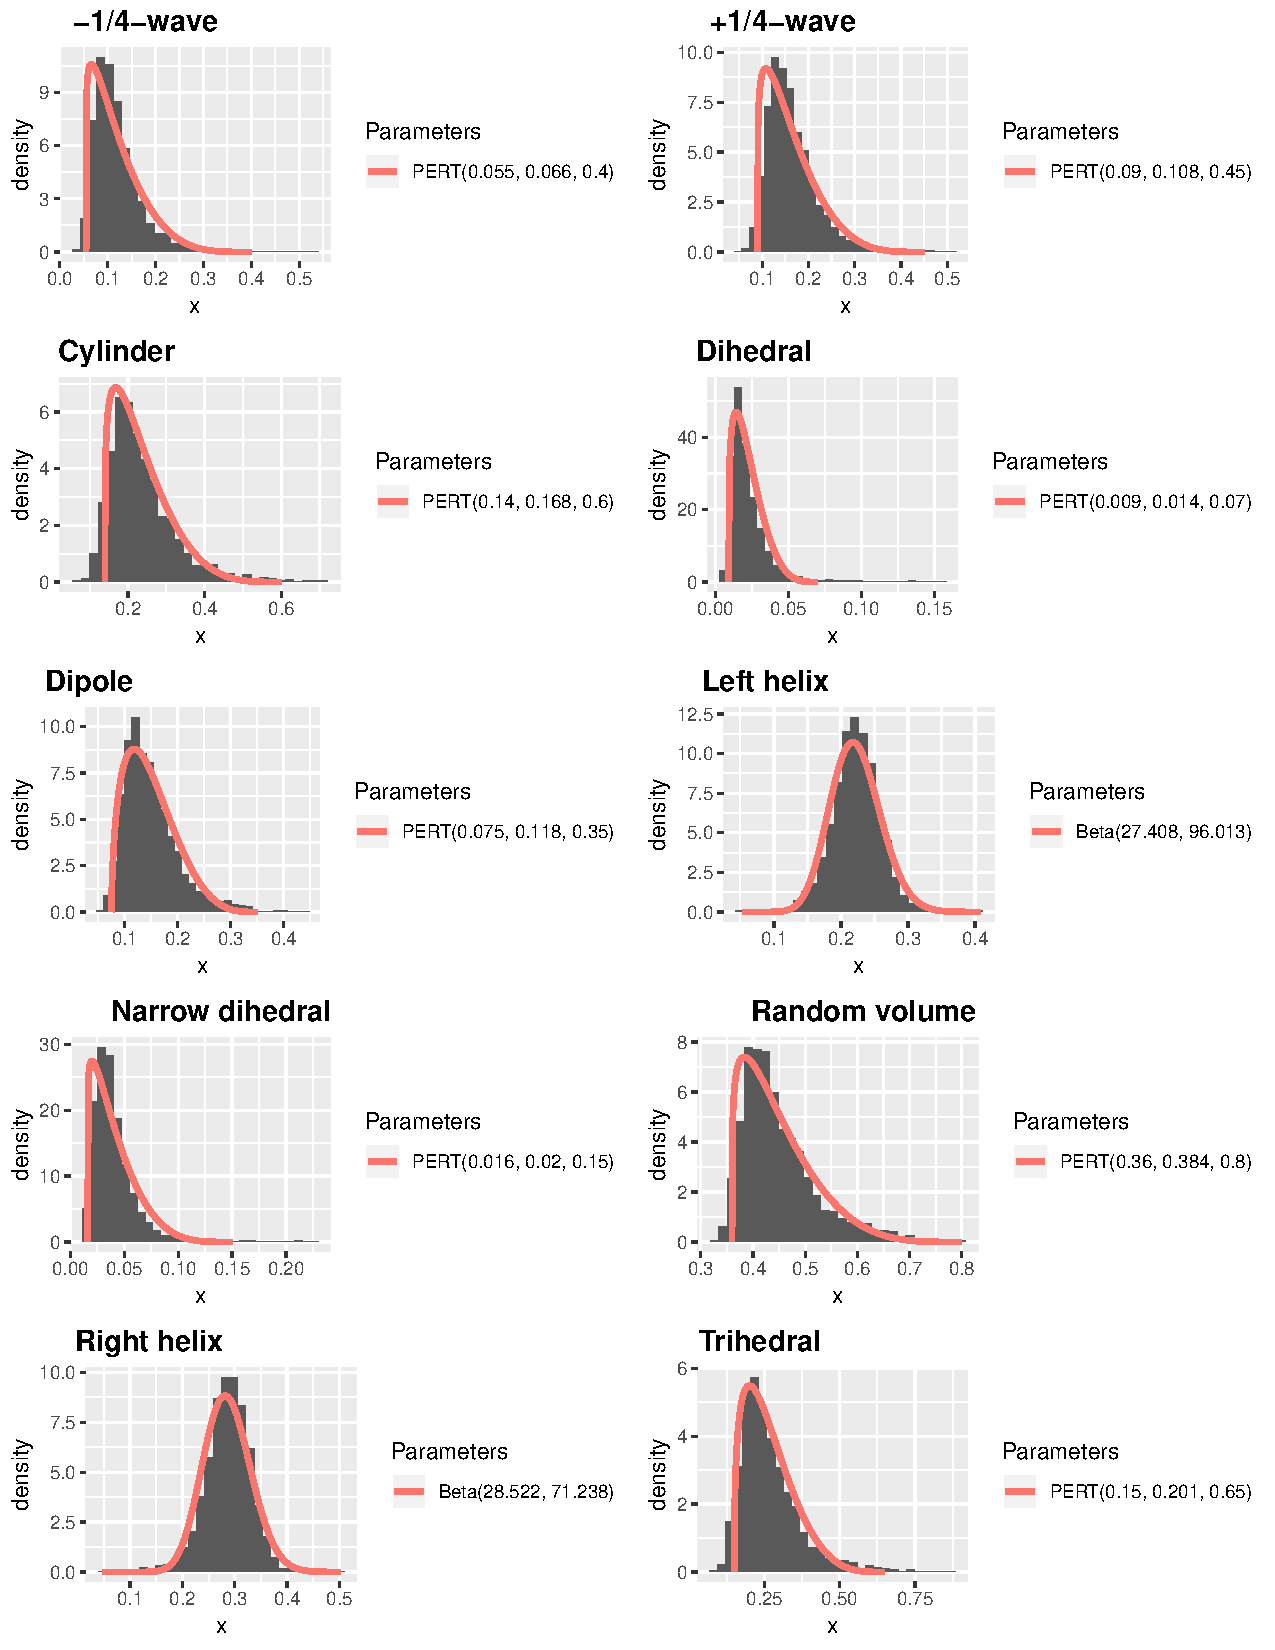
\includegraphics[width = 0.8\linewidth]{../../Figures/Report_19_02_27/region4_plots.pdf}
  \caption{Histogramas referentes às similaridades dos dados da região 4 em relação aos retroespalhadores elementares}
  \label{fig:hists4}

\end{figure}

\section{Conclusão}

Analisando os resultados dispostos no presente relatório, concluí-se que a similaridade dos dados de regiões de solo exposto em relação ao retroespalhador prototípico \textit{random volume} apresenta um comportamento estatístico que pode ser modelado por uma distribuição de probabilidade e que difere do comportamento observado em regiões com alguma vegetação. Portanto, é possível distinguir regiões de solo exposto de regiões com vegetação por meio da Distância Geodésica de seus dados a \textit{random volume}.

Os próximos passos consistirão em
\begin{itemize}
  \item reproduzir as análises realizadas para dados de campo com qualidade assegurada;
  \item observar o comportamento da similaridade dos dados de outros tipos de regiões.
\end{itemize}
\end{document}